%% Template para dissertacao/tese na classe UFBAthesis
%% versao 1.0
%% (c) 2005 Paulo G. S. Fonseca
%% (c) 2012 Antonio Terceiro
%% (c) 2014 Christina von Flach
%% www.dcc.ufba.br/~flach/ufbathesis

%% Carrega a classe ufbathesis
%% Opcoes: * Idiomas
%%           pt   - portugues (padrao)
%%           en   - ingles
%%         * Tipo do Texto
%%           bsc  - para monografias de graduacao
%%           msc  - para dissertacoes de mestrado (padrao)
%%           qual - exame de qualificacao de mestrado
%%           prop - exame de qualificacao de doutorado
%%           phd  - para teses de doutorado
%%         * Media
%%           scr  - para versao eletronica (PDF) / consulte o guia do usuario
%%         * Estilo
%%           classic - estilo original a la TAOCP (deprecated) - apesar de deprecated, manter esse.
%%           std     - novo estilo a la CUP (padrao)
%%         * Paginacao
%%           oneside - para impressao em face unica
%%           twoside - para impressao em frente e verso (padrao)

% Atenção: Manter 'classic' na declaracao abaixo:
\documentclass[qual, classic, a4paper]{ufbathesis}

%% Preambulo:
\usepackage[utf8]{inputenc}

%\usepackage[authoryear]{natbib}
\usepackage{graphicx}
\usepackage{lipsum}
\usepackage{hyphenat}
\usepackage[usenames, dvipsnames, table]{xcolor}
\usepackage{booktabs}
\usepackage{pifont}
\usepackage{multirow}
\usepackage{listings} 
\usepackage{colortbl}
\usepackage{xfrac}
\usepackage[FIGTOPCAP]{subfigure}
\usepackage{tabularx}
\usepackage{ragged2e}
\usepackage{acronym}
\usepackage{float}
\usepackage{todonotes}



% Siglas
\acrodef{AM}[AM]{{Aprendizado de Máquina}}
\acrodef{EMD}[EMD]{{Decomposição de Modo Empírico}}
\acrodef{RQA}[RQA]{{\textit{Recurrence Quantification Analysis}}}
 \acrodef{FAPAR}[FAPAR] {{\textit{Fraction of Absorbed Photosynthesis Active Radiation}}}
 \acrodef{DTW}[DTW] {{\textit {Dynamic  Time  Warping}}}
 \acrodef{DE}[DE] {{Distância Euclidiana}}
 \acrodef{EDR}[EDR]{{ \textit{ Edite  Distance  Real}}}
\acrodef{CID}[CID]{{\textit{Complexity-Invariant Distance}}}
\acrodef{SLR}[SLR]{{\textit{Systematic  Literature  Review}}}
\acrodef{SANTS}[SANTS]{{\textit{Similarity Analysis on Nonstationary Time Series}}} 
\acrodef{MDDL}[MDDL]{{\textit{Mean Distance from the Diagonal Line}}}


% Universidade
\university{Universidade Federal da Bahia}

% Endereco (cidade)
\address{Salvador}

% Instituto ou Centro Academico
\institute{Instituto de Matem\'{a}tica}

% Nome da biblioteca - usado na ficha catalografica
\library{Biblioteca Reitor Mac\^{e}do Costa}

% Programa de pos-graduacao
\program{Programa de P\'{o}s-Gradua\c{c}\~{a}o em Ci\^{e}ncia da Computa\c{c}\~{a}o}

% Area de titulacao
\majorfield{Ci\^{e}ncia da Computa\c{c}\~{a}o}

% Titulo da dissertacao
\title{Detecção de Novidades em Stream de Dados utilizandos funções de base radial e cadeias de Markov}

% Data da defesa
% e.g. \date{19 de fevereiro de 2013}
\date{03 de Abril de 2019}
% e.g. \defenseyear{2013}
\defenseyear{2019}

% Autor
% e.g. \author{Jose da Silva}
\author{Ruivaldo Azevedo Lobão Neto}

% Orientador(a)
% Opcao: [f] - para orientador do sexo feminino
% e.g. \adviser[f]{Profa. Dra. Maria Santos}
\adviser{Ricardo Ara\'{u}jo Rios}

% Orientador(a)
% Opcao: [f] - para orientador do sexo feminino
% e.g. \coadviser{Prof. Dr. Pedro Pedreira}
% Comente se nao ha co-orientador
%\coadviser{Nome Completo do CO-ORIENTADOR}

%% Inicio do documento
\begin{document}

\pgcompfrontpage

%% Parte pre-textual
\frontmatter

\pgcomppresentationpage

%%%%%%%%%%%%%%%%%%%%%%%%%
% Ficha catalografica
%%%%%%%%%%%%%%%%%%%%%%%%%

%\authorcitationname{Silva, Mirlei Moura da } % e.g. Terceiro, Antonio Soares de Azevedo
%\advisercitationname{Sobrenome, Nome do ORIENTADOR} % e.g. Chavez, Christina von Flach Garcia
%\coadvisercitationname{Sobrenome, Nome do CO-ORIENTADOR} % e.g. Mendonca, Manoel Gomes de
%\catalogtype{Disserta\c{c}\~{a}o (Mestrado)} % e.g. ou ``Tese (Doutorado)''

%\catalogtopics{1. Primeira palavra-chave. 2. Segunda palavra-chave. 3. Terceira palavra-chave} % Listar palavras-chave do trabalho para a FICHA CATALOGRAFICA}, por exemplo, ``1. Complexidade Estrutural. 2. Qualidade de Software 3. Engenharia de Software''
%\catalogcdd{XXX.XX} % e.g.  XXX.XX (número nesse formato serah dado pela biblioteca)
%\catalogcdu{XXX.XX.XXX} % e.g.  XXX.XX.XXX (idem) 
%\catalogingsheet

%%%%%%%%%%%%%%%%%%%%%
% Termo de aprovacaoo
%%%%%%%%%%%%%%%%%%%%%

\approvalsheet{Salvador, 03 de Abril de 2019}{
   \comittemember{Prof. Dr. Ricardo Araújo Rios}{UFBA}  
   %\comittemember{Profa. Dr...}{UFBA}
   %\comittemember{Prof. Dr...}{USP} 
}
   % Para mestrado, apenas 3.
   % \comittemember{Prof. Dr. Professor 4}{Universidade HJKL}
   % \comittemember{Profa. Dra. Professora 5}{Universidade QWERTY}

%%%%%%%%%%%%%%%%%%%%%%%%%%%%%%%%%%%%%%%% 
% Dedicatoria, Agradecimentos, Epigrafe
%%%%%%%%%%%%%%%%%%%%%%%%%%%%%%%%%%%%%%%%

% Comente para ocultar
%\begin{dedicatory}
%DIGITE A DEDICATORIA AQUI
%\end{dedicatory}

% Agradecimentos
% Se preferir, crie um arquivo `a parte e o inclua via \include{}
%\acknowledgements
%DIGITE OS AGRADECIMENTOS AQUI

% Epigrafe
%\begin{epigraph}[NOTA]{AUTOR}
%DIGITE AQUI A CITACAO
%\end{epigraph}

%%%%%%%%%%%%%%%%%%%%%
% Resumo 
%%%%%%%%%%%%%%%%%%%%%
\resumo

% Com a grande quantidade dados produzidos e coletados diariamente por diferentes sistemas, 
% técnicas de aprendizado de máquina foram propostas com o intuito de auxiliar no processo de 
% extração automática de informações. 
% Dentre essas técnicas, pode-se destacar os algoritmos de agrupamento que buscam encontrar 
% padrões e estruturas implícitas em conjuntos de dados sem qualquer conhecimento fornecido à 
% priori. Neste trabalho de mestrado, busca-se desenvolver uma nova abordagem de agrupamento 
% para dados que possuem uma dependência temporal entre suas observações, comumente 
% chamados de séries temporais. A principal diferença dessa abordagem em relação aos 
% trabalhos existentes na literatura baseia-se na hipótese de que dados coletados do 
% mundo real possuem influências estocásticas e determinísticas que, se não forem 
% individualmente analisadas, podem afetar o resultado do agrupamento. 
% Neste sentido, a abordagem proposta realiza uma etapa de decomposição das séries 
% temporais em componentes estocásticos e determinísticos. Em seguida, realiza o 
% agrupamento dos dados analisando de maneira individual a similaridade entre cada componente. 
% Experimentos preliminares foram realizados sobre séries temporais sintéticas, 
% formadas a partir da combinação entre componentes estocásticos e determinísticos. 
% A partir da decomposição das séries sintéticas, 
% foi possível observar que medidas de distância largamente utilizadas na literatura 
% apresentaram melhores resultados. 
% Ao afinal deste trabalho de mestrado, espera-se obter um melhor resultado de agrupamento 
% utilizando a abordagem proposta sobre dados reais.

\vspace{1cm}

A mudança e o desenvolvimento contínuos são aspectos essenciais dos ambientes em evolução e
aplicações, incluindo, mas não limitado a cidades inteligentes, militares, medicina, reatores nucleares,
carros autônomos, aviação e indústria aeroespacial. Ou seja, as características fundamentais de tais
ambientes podem evoluir, e assim causar conseqüências perigosas, por exemplo, colocando vidas humanas em risco, se nenhuma reação for adotada. Portanto, os sistemas de aprendizagem precisam aplicar
algoritmos para monitorar a evolução em seus ambientes e atualizar-se efetivamente.

Na literatura sobre aprendizado de máquina, o fenômeno da mudança (distributiva) nos dados
é conhecido como \textit{concept drift}. A sua ocorrência pode mudar os limites da decisão e causar um declínio
na precisão do modelo. Os algoritmos de aprendizado precisam detectar o \textit{concept drift} nos fluxos de dados e substituir ou atualizar seus modelos preditivos adequadamente. Para enfrentar esse desafio, foram concebidos métodos de detecção de \textit{concept drift} em fluxos de dados dinâmicos e variáveis. Um método de detecção ideal deve identificar mudanças de conceito rapidamente, com as menores taxas de falso positivo e falso negativo.
Falso positivo refere-se a incorretamente identificar um \textit{concept drift}, e falso negativo se refere a não
identificar um \textit{concept drift} quando é devido.

\todo{Termina resumo...}

% Palavras-chave do resumo em Portugues
\begin{keywords}
    Ambiente com fluxo contínuo de dados (\textit{Data stream}); Mudanças de conceito (\textit{Concept drift}); Métodos de detecção de mudanças (\textit{Concept drift detection})
\end{keywords}

%\input abstract

%%%%%%%%%%%%%%%%%%%
% Sumario / Indice
%%%%%%%%%%%%%%%%%%%

% Comente para ocultar
\tableofcontents

% Lista de figuras
% Comente para ocultar
\listoffigures

% Lista de tabelas
% Comente para ocultar
\listoftables

%% Parte textual
\mainmatter

% Eh aconselhavel criar cada capitulo em um arquivo separado, digamos
% "capitulo1.tex", "capitulo2.tex", ... "capituloN.tex" e depois
% inclui-los com:
% \include{capitulo1}
% \include{capitulo2}
% ...
% \include{capituloN}
%
% Importante: 
% Use \xchapter{}{} ao inves de \chapter{}; se não quiser colocar texto antes do inicio do capitulo, use \xchapter{texto}{}.

% Introdução
\xchapter{Introdu\c{c}\~{a}o}{}\label{introducao}

\section{Considerações Iniciais}

Atualmente, grandes volumes de dados são coletados e produzidos por diferentes sistemas. Segundo \citeonline{Nguyen2015}, diariamente, mais de 3,5 bilhões de buscas são realizadas nos repositórios do Google e cerca de de 4TB de imagens são geradas por satélites da NASA. 

Além das grandes corporações, com o surgimento das redes sociais e a populariazação de dispositivos de acesso à Internet, usuários comuns passaram a produzir, de maneira efetiva, grandes volumes de dados por meio, por exemplo, da publicação e compartilhamento de fotos, textos e vídeos.

Por fim, é importante destacar que evoluções em áreas estratégicas da computação têm favorecido o crescente aumento no volume de dados produzidos e armazenados. Uma dessas áreas é chamada de Internet das Coisas  (\textit{Internet of Things}) \cite{iot}, a qual visa conectar e coordenar diferentes dispositivos sem a intervenção humana. Recentemente, uma pesquisa divulgada pela IDC (\textit{International Data Corporation})  apresentou uma previsão de que cerca de 32 bilhões de dispositivos estarão interconectados até 2020 \cite{iot}. 

Esse aumento significativo na quantidade de dados produzidos e armazenados tem dificultado a tarefa de especialistas de domínio na análise e extração novas informações. Visando superar essas dificuldades, técnicas de \ac{AM} têm sido propostas para desenvolver programas de computadores que sejam capazes de analisar dados e aprender, com base na experiência fornecida por especialistas, com intuito de melhorar o desempenho na realização de alguma tarefa \cite{Mitchell:1997:ML:541177,faceli2011inteligencia}. 

De maneira geral, o aprendizado realizado por técnicas de \ac{AM} ocorre visando induzir hipóteses que sejam capazes de descrever relações entre os dados analisados. Essa busca por tais hipóteses é determinada pelo viés de cada algoritmo, o qual representa a capacidade de generalização do modelo aprendido quando aplicado à novos dados não vistos previamente \cite{faceli2011inteligencia}.

Ao encontrar hipóteses que descrevem o comportamento dos dados, pode-se ajustar um modelo para, por exemplo, predizer o comportamento futuro de um sistema ou, simplesmente, descrever seu estado atual. O ajuste destes modelos ocorre de acordo com o paradigma de aprendizado, o qual pode ser supervisionado ou não-supervisionado. No paradigma supervisionado, modelos são estimados considerando um conjunto de instâncias (dados) que contém características (atributos) específicas de cada instância (dado) e um rótulo (atributo meta), o qual é normalmente fornecido por um especialista. Tarefas de aprendizagem neste caso são, geralmente, realizadas para classificação e regressão de novas instâncias.

Por outro lado, existem situações onde não é possível contar com um especialista para, previamente, fornecer rótulos para cada instância. Neste caso, a utilização de métodos de aprendizagem do paradigma não-supervisionado são normalmente utilizados, uma vez que nenhuma informação é conhecida a priori, exceto os atributos de cada instância.

Dentre as técnicas do paradigma não-supervisionado mais utilizadas na literatura, pode-se destacar os algoritmos de Agrupamento de Dados. Esses algoritmos analisam dados buscando estruturas de tal forma que dados pertencentes a um mesmo grupo sejam de alguma forma mais semelhantes do que dados de outros grupos \cite{Mitchell:1997:ML:541177,faceli2011inteligencia, Aghabozorgi2015}.

Os dados analisados pelos algoritmos de agrupamento podem  ser caracterizados de diferentes formas como, por exemplo:  textos em redes sociais, cadastro de clientes de uma organização, ou exames realizados em pacientes de um hospital. 

Em geral, dados são coletados de maneira independente e identicamente distribuída (iid), ou seja, são coletados seguindo alguma distribuição de probabilidade sem, necessariamente, ser caracterizado por uma dependência temporal. Entretanto, quando existe essa dependência, dados são organizados como séries temporais \cite{Esling2012,box2015}. Por exemplo, séries temporais podem ser utilizadas para representar medidas sequenciais ao longo do tempo de médias diárias de temperatura de uma cidade, variações de preço de uma determinada ação na bolsa de valores, propagação de uma doença ou cantos de pássaros \cite{Esling2012}. 

Assim, o foco deste trabalho de mestrado é analisar a aplicação de técnicas de agrupamento de dados em séries temporais. Visando apresentar claramente as contribuições deste trabalho, a próxima seção detalha o contexto e a motivação para realização dessa análise.

\section{Contextualização e Motivação}

Séries temporais são representadas por uma coleção de valores obtidos a partir de medidas sequenciais ao longo do tempo e são utilizadas para análise do comportamento de sistemas em diversas áreas, tais como a medicina, meteorologia, captura de movimento, governo, engenharia, negócios, finanças, economia, entre outras \cite{Esling2012,box2015}. 

O agrupamento de séries temporais possibilita extrair informações em conjuntos de dados temporais, agrupando as séries (instâncias) em grupos (\textit{clusters}) de tal forma que a variância \textit{intercluster} seja maximizada e a \textit{intracluster} seja minimizada. Assim, séries que compartilham características (informações) similares são organizadas em um mesmo grupo.

Para determinar variâncias entre séries temporais são utilizadas métricas que calculam similaridades~\cite{Mori2016}. Na literatura de aprendizado de máquina não-supervisionado, instâncias são agrupadas considerando métricas de similaridades ou métricas de distância. Em algumas situações, a similaridade entre duas instâncias pode ser calculada utilizando o inverso da distância entre elas. 

No entanto, a escolha de tais métricas não é trivial, uma vez que séries temporais podem apresentar diferentes comportamentos que influenciam o cálculo da similaridade. Por exemplo, a similaridade entre séries com comportamento determinístico pode ser calculada utilizando técnicas como \ac{DTW} \cite{tormene2009matching} ou \ac{MDDL} \cite{Araujo2015, Araujo2013}.Por outro lado, o cálculo da similaridade entre séries com comportamento estocástico pode ser realizado a partir da análise no domínio de frequência, i.e., comparando espectrogramas obtidos com a transformada de Fourier~\cite{morettin2006}.

Contudo, séries temporais podem apresentar uma mistura de ambos os comportamentos. Conforme discutido em~\citeonline{Araujo2013,Araujo2015}, considerar apenas um dos comportamentos pode reduzir a acurácia no processo de modelagem e análise de séries temporais.

Visando resolver essa limitação, este projeto de mestrado discute uma abordagem que permite analisar individualmente os comportamento estocásticos e determinísticos no processo de cálculo de similaridade entre séries temporais e, consequentemente, melhorar o processo de agrupamento de dados.

\section{Hipótese e Objetivo}

Com base nas observações citadas anteriormente, a seguinte hipótese foi formulada:

\begin{center}
\textit{``O agrupamento de séries temporais apresenta maior acurácia quando medidas de similaridade (ou distância) são, individualmente, calculadas sobre comportamentos estocásticos e determinísticos.''}
\end{center}

Assim, o objetivo deste trabalho de mestrado será validar esta hipótese. Para alcançar esse objetivo, será desenvolvida uma abordagem de agrupamento que decompõe séries temporais em dois componentes, um estocástico e um determinístico. Inicialmente, a decomposição das séries será realizada considerando as abordagens propostas em \citeonline{Araujo2013,Araujo2015}. A partir dessa decomposição, será possível, individualmente, medir a similaridade/distância entre cada componente. Para isso, diferentes métricas de similaridade e distância serão implementadas para validação da abordagem proposta. As séries utilizadas nos experimentos serão divididas em dois conjuntos. Um conjunto formado por séries sintéticas, que permitirá realizar uma análise detalhada da abordagem, uma vez que os comportamentos estocásticos e determinísticos serão previamente conhecidos. O outro conjunto será composto por séries coletadas de algum sistema do mundo real, visando apresentar uma aplicação prática para a solução proposta neste trabalho.

O restante deste projeto  está organizado da seguinte maneira: O \textbf{Capítulo \ref{revisao}} possui uma revisão bibliográfica dos principais conceitos utilizados neste trabalho como, por exemplo, análise, decomposição e agrupamento de séries temporais; No \textbf{Capítulo \ref{plano}} está o plano de pesquisa elaborado com o objetivo de validar a hipótese desta pesquisa, a metodologia que será utilizada na pesquisa e o cronograma de atividades; finalmente, no \textbf{Capítulo \ref{experimentos}}, é apresentado um conjunto de experimentos preliminares, os quais foram desenvolvidos para demonstrar a importância de analisar os comportamentos estocásticos e determinísticos no agrupamento de séries temporais.
% /Introdução

\input revisao

\input plano

\input experimentos


%% Parte pos-textual
\backmatter

% Bibliografia
% É aconselhável utilizar o BibTeX a partir de um arquivo, digamos "biblio.bib".
% Para ajuda na criação do arquivo .bib e utilização do BibTeX, recorra ao
% BibTeXpress em www.cin.ufpe.br/~paguso/bibtexpress
\bibliographystyle{abntex2-alf}
\bibliography{biblio}

% Apendices
% Comente se naoo houver apendices
%\appendix

%\xchapter{Exemplo de Ap\^endice}{} %sem preambulo
%\lipsum
% Eh aconselhavel criar cada apendice em um arquivo separado, digamos
% "apendice1.tex", "apendice.tex", ... "apendiceM.tex" e depois
% inclui--los com:
%\xchapter{Decomposição das séries temporais}{} %sem preambulo
\label{apendice1}
\section{Considerações Iniciais}
Neste apêndice consta as 40 séries temporais utilizadas nos experimentos mostrados no Capitulo \ref{experimentos}. As séries foram divididas em 4 tipos conforme a Tabela \ref{series}, onde o tipo representa um conjunto de 10 séries senoide ou cossenoide, sendo acrescida de ruído ou acrescida de ruído e tendência.
Nas imagens são representadas, a séries original,   seu componente determinístico e seu componente estocástico, os quais foram extraídos após a decomposição.
\section{Séries TIPO 1}
10 séries cossenoide com ruído ao longo da série.
\graphicspath{{imagens/}}
\begin{figure}[H]
\begin{center}
  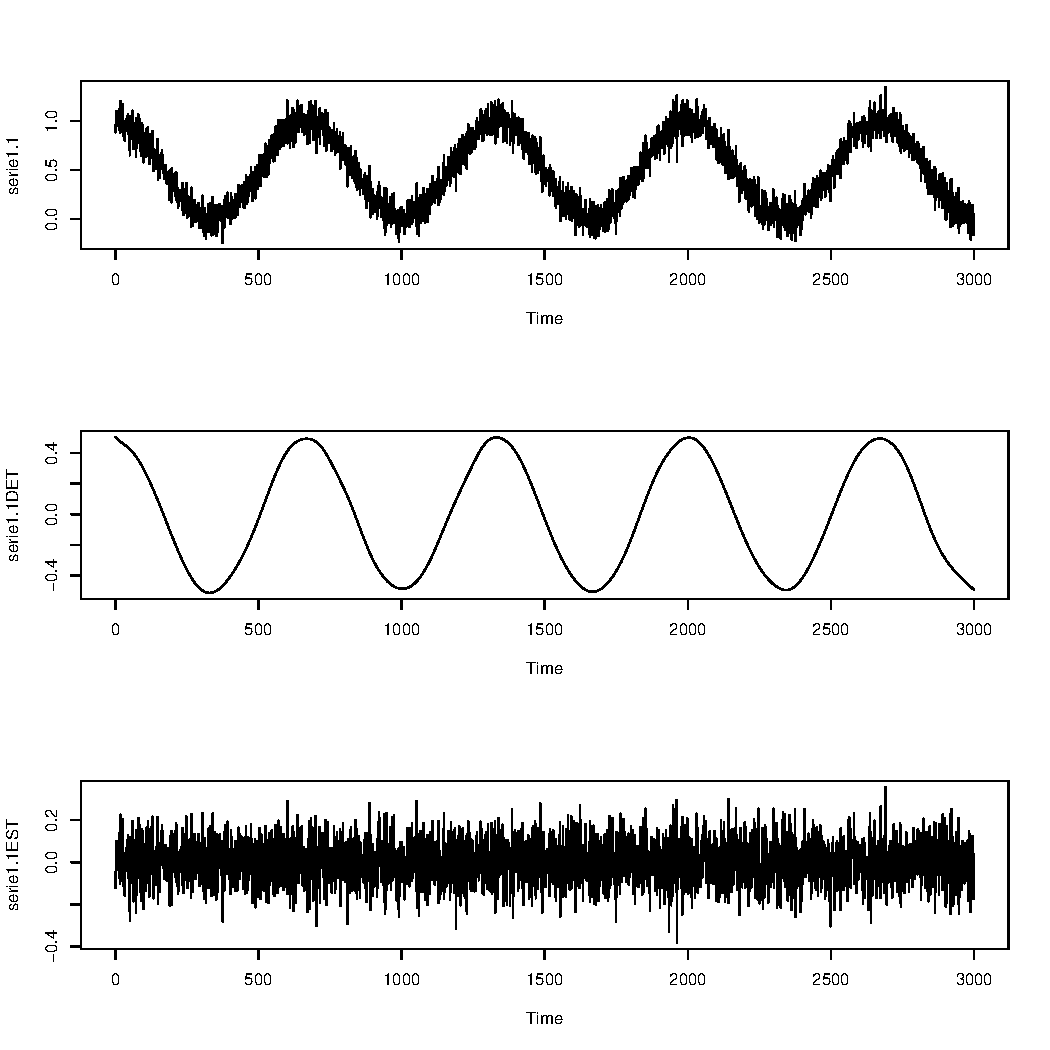
\includegraphics[scale=0.43]{serie1_1.pdf} \quad
  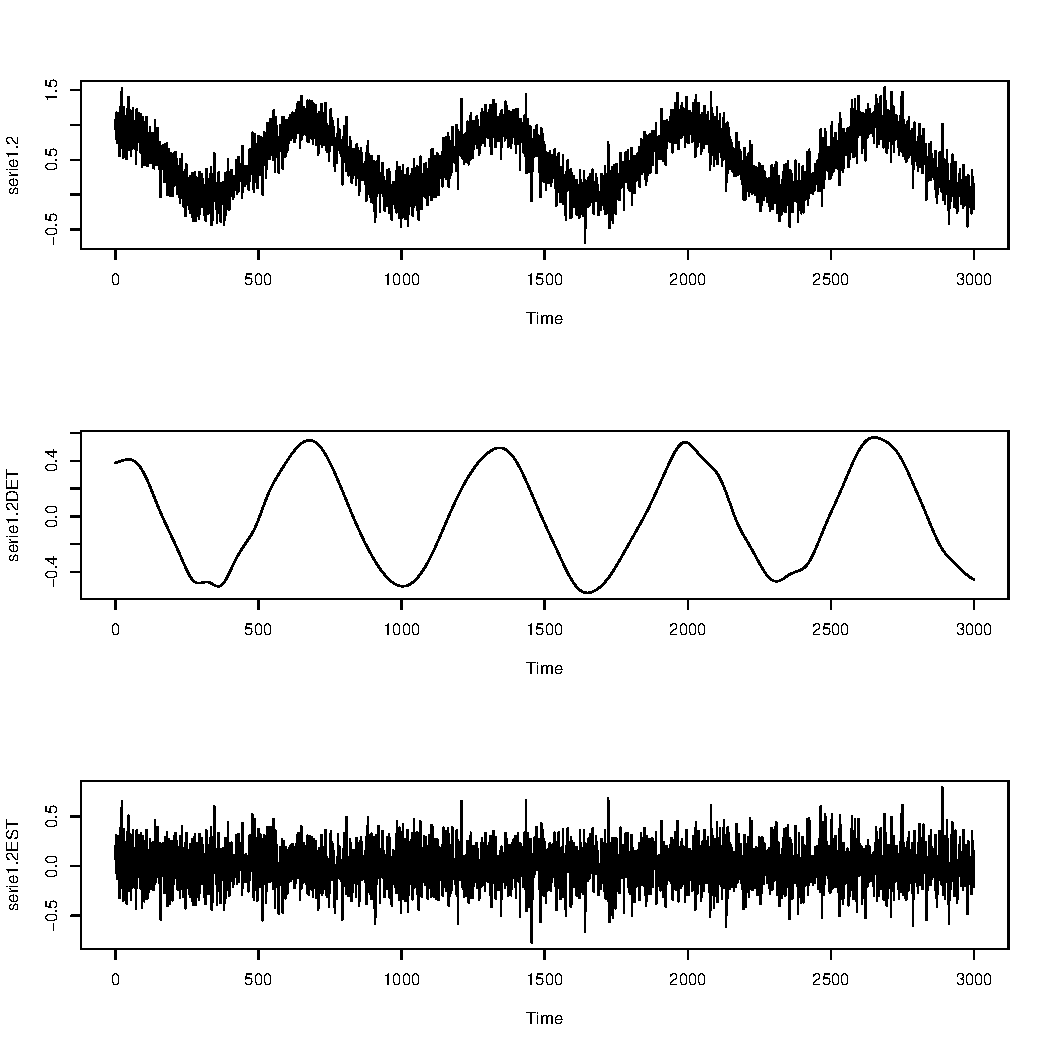
\includegraphics[scale=0.43]{serie1_2.pdf}
  \caption{Série 1.1 e Série 1.2}

\end{center}
\end{figure}

\graphicspath{{imagens/}}
\begin{figure}[H]
\begin{center}
  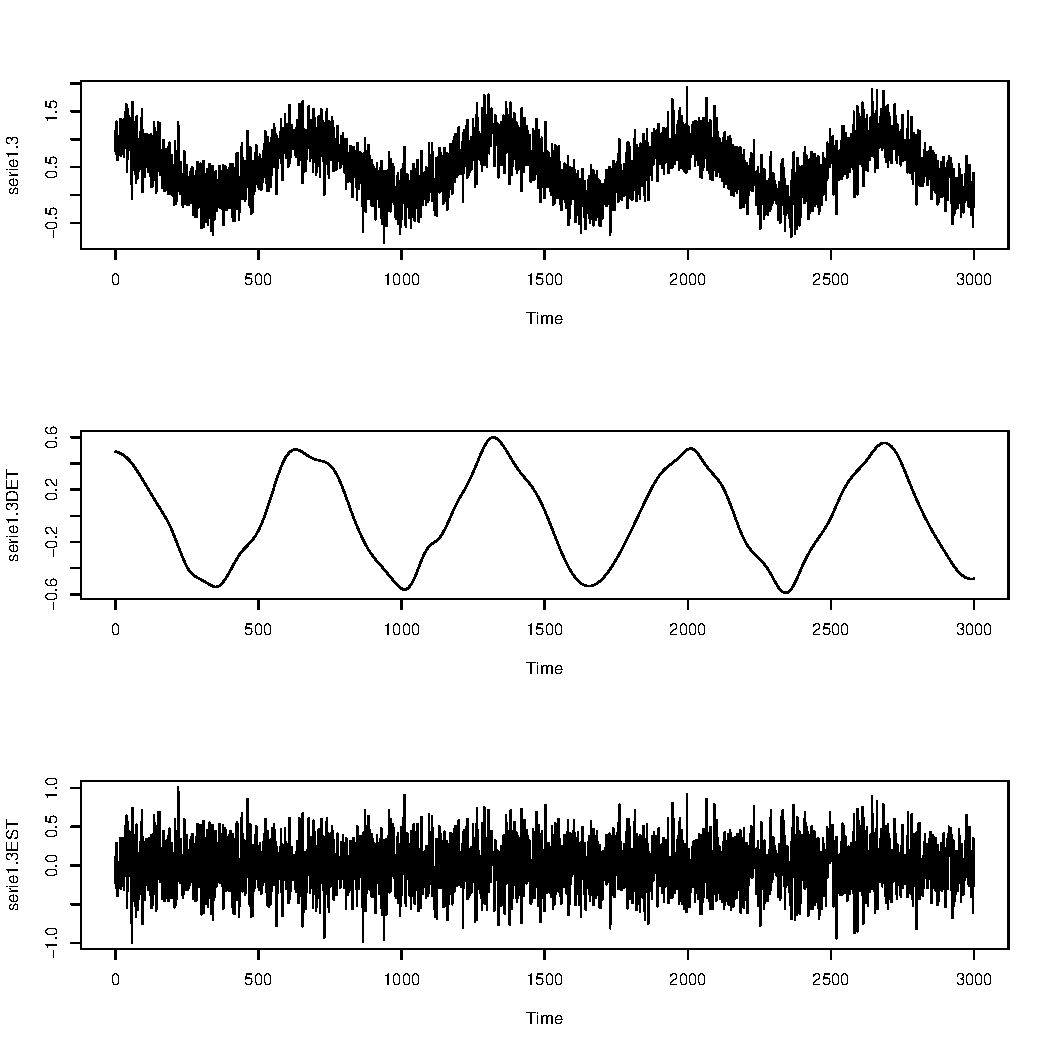
\includegraphics[scale=0.43]{serie1_3.pdf} \quad
  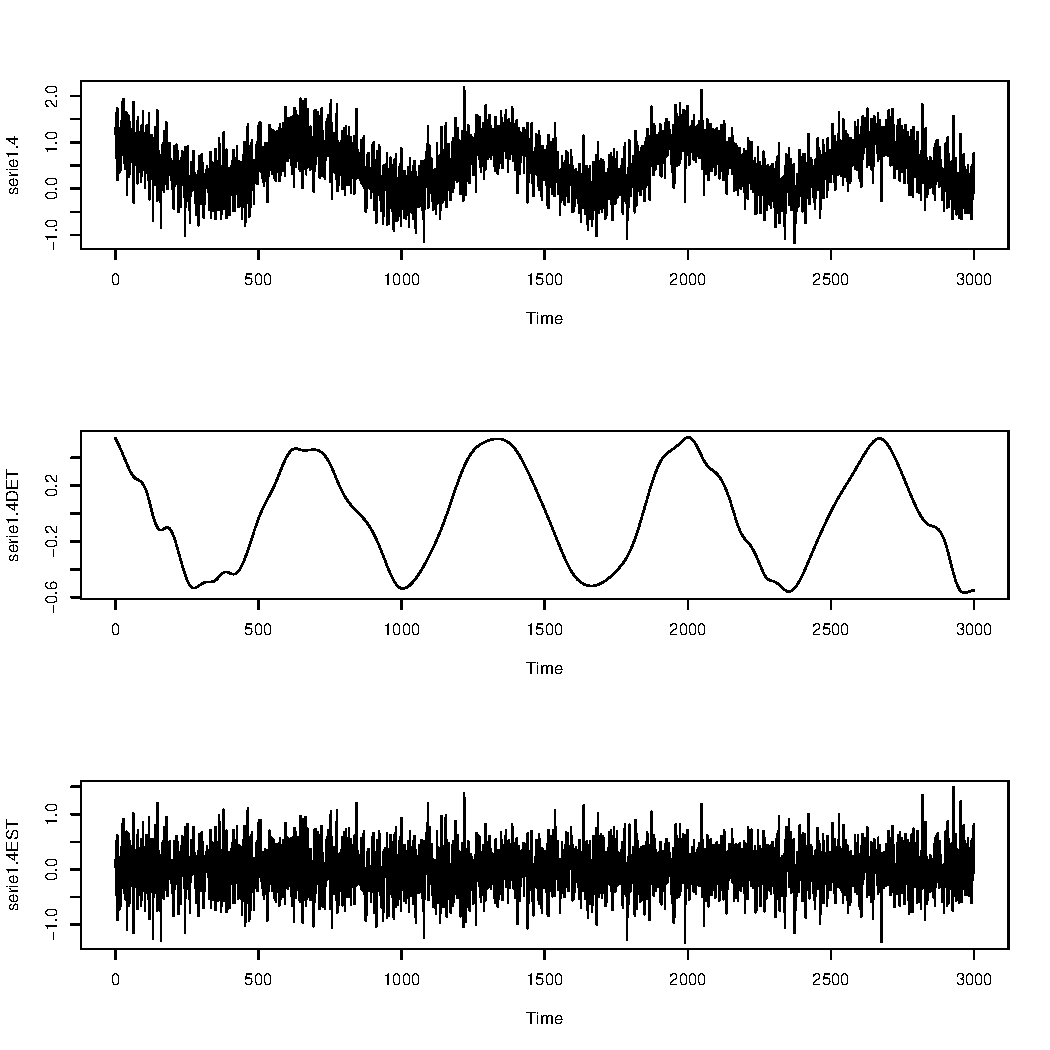
\includegraphics[scale=0.43]{serie1_4.pdf}
  \caption{Série 1.3 e Série 1.4}

\end{center}
\end{figure}

\graphicspath{{imagens/}}
\begin{figure}[H]
\begin{center}
  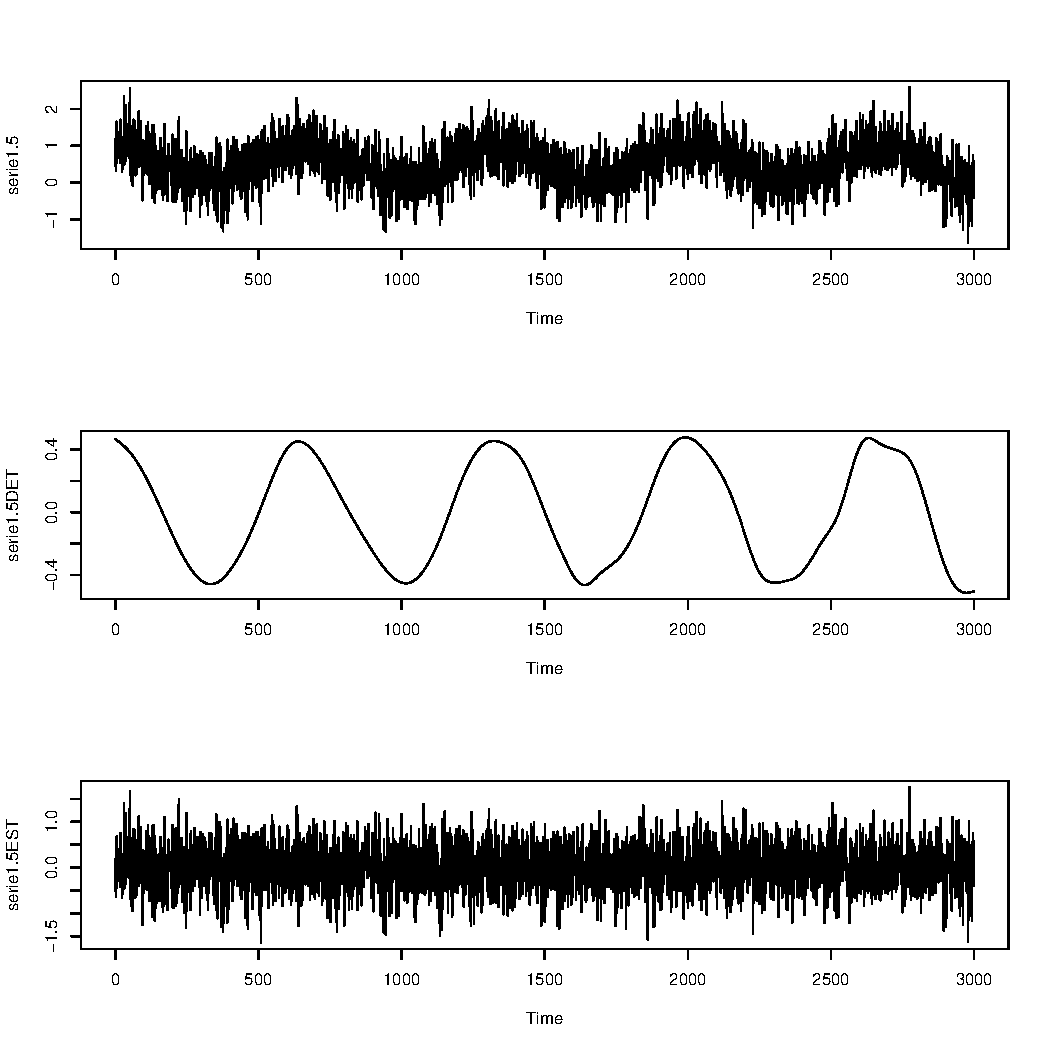
\includegraphics[scale=0.43]{serie1_5.pdf} \quad
  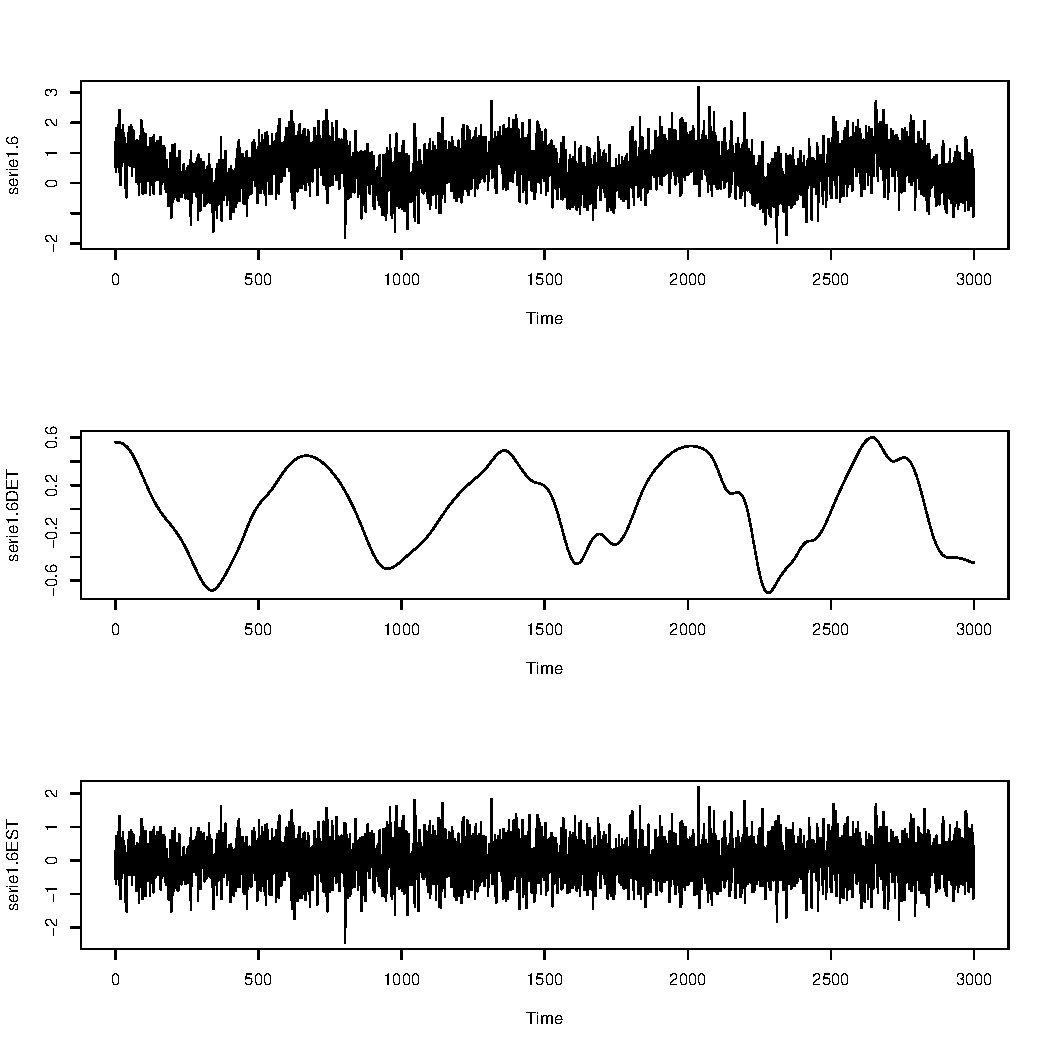
\includegraphics[scale=0.43]{serie1_6.pdf}
  \caption{Série 1.5 e Série 1.6}

\end{center}
\end{figure}

\graphicspath{{imagens/}}
\begin{figure}[H]
\begin{center}
  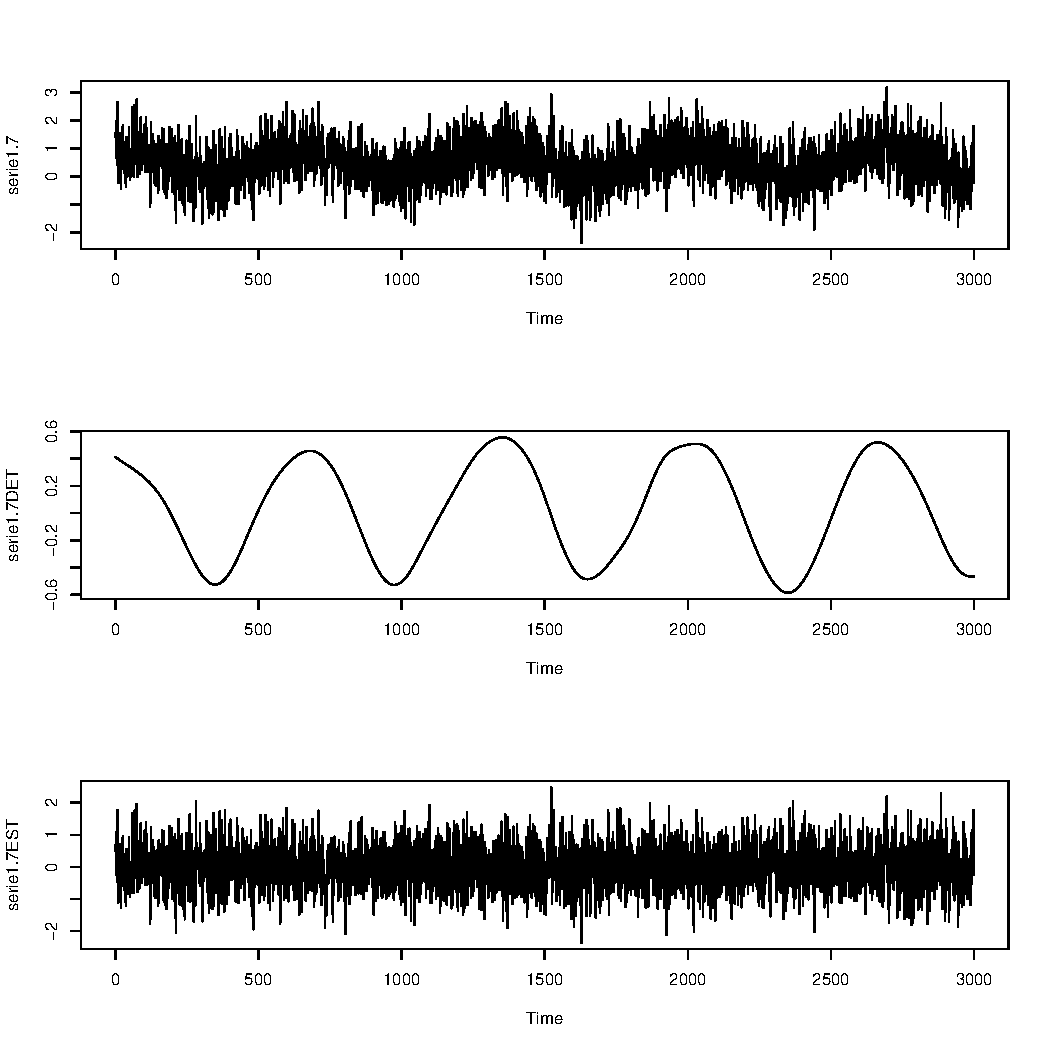
\includegraphics[scale=0.43]{serie1_7.pdf} \quad
  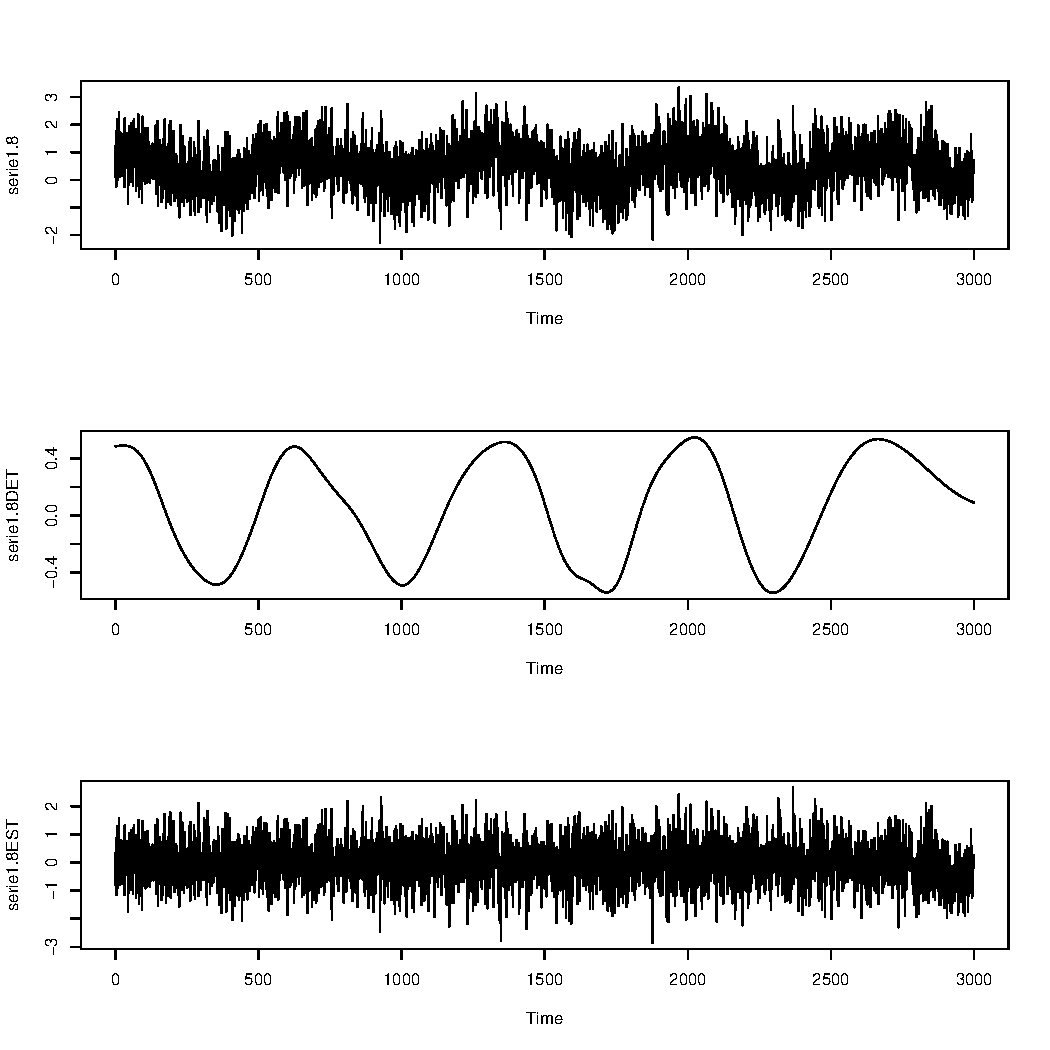
\includegraphics[scale=0.43]{serie1_8.pdf}
  \caption{Série 1.7 e Série 1.8}

\end{center}
\end{figure}

\graphicspath{{imagens/}}
\begin{figure}[H]
\begin{center}
  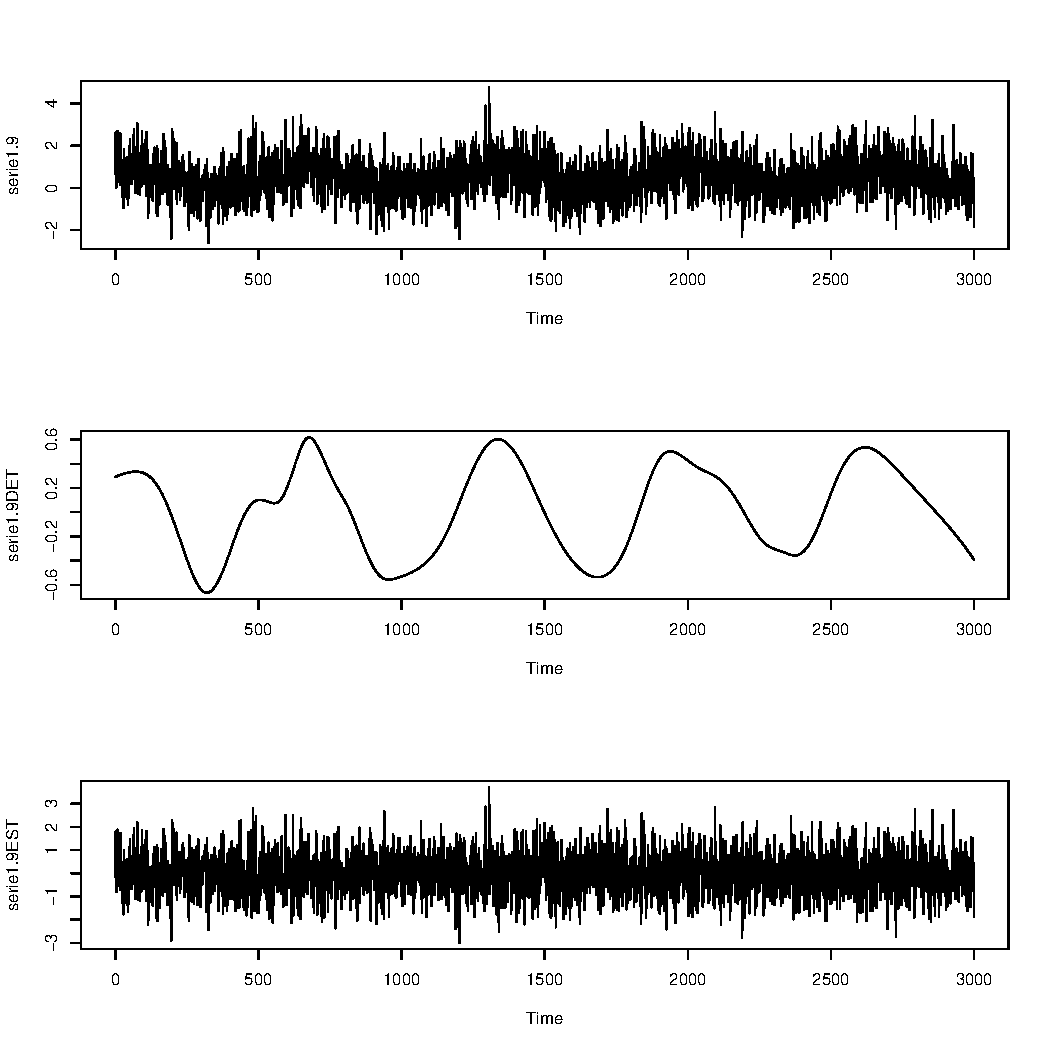
\includegraphics[scale=0.43]{serie1_9.pdf} \quad
  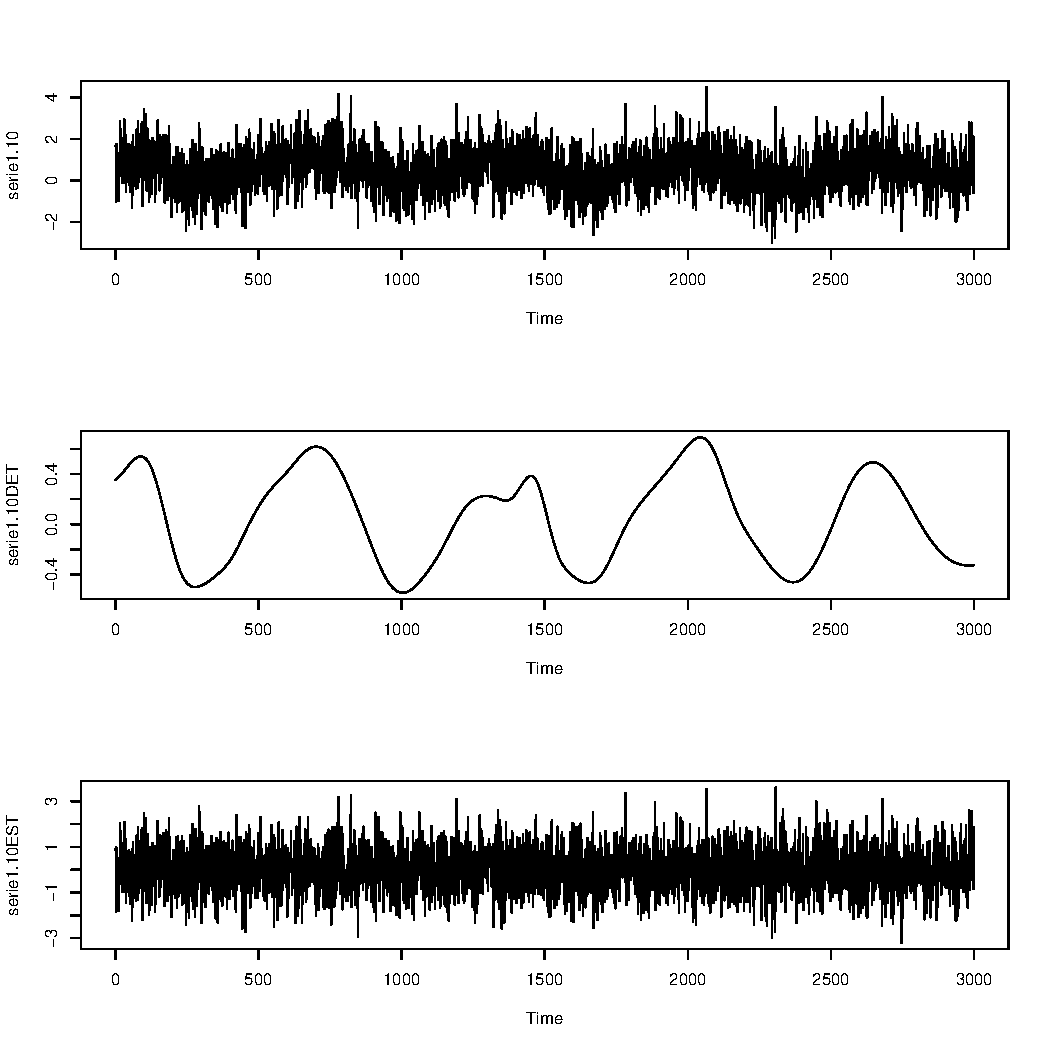
\includegraphics[scale=0.43]{serie1_10.pdf}
  \caption{Série 1.9 e Série 1.10}

\end{center}
\end{figure}

\section{Séries TIPO 2}
10 séries cossenoide com ruído ao longo da série e tendência.
\graphicspath{{imagens/}}
\begin{figure}[H]
\begin{center}
  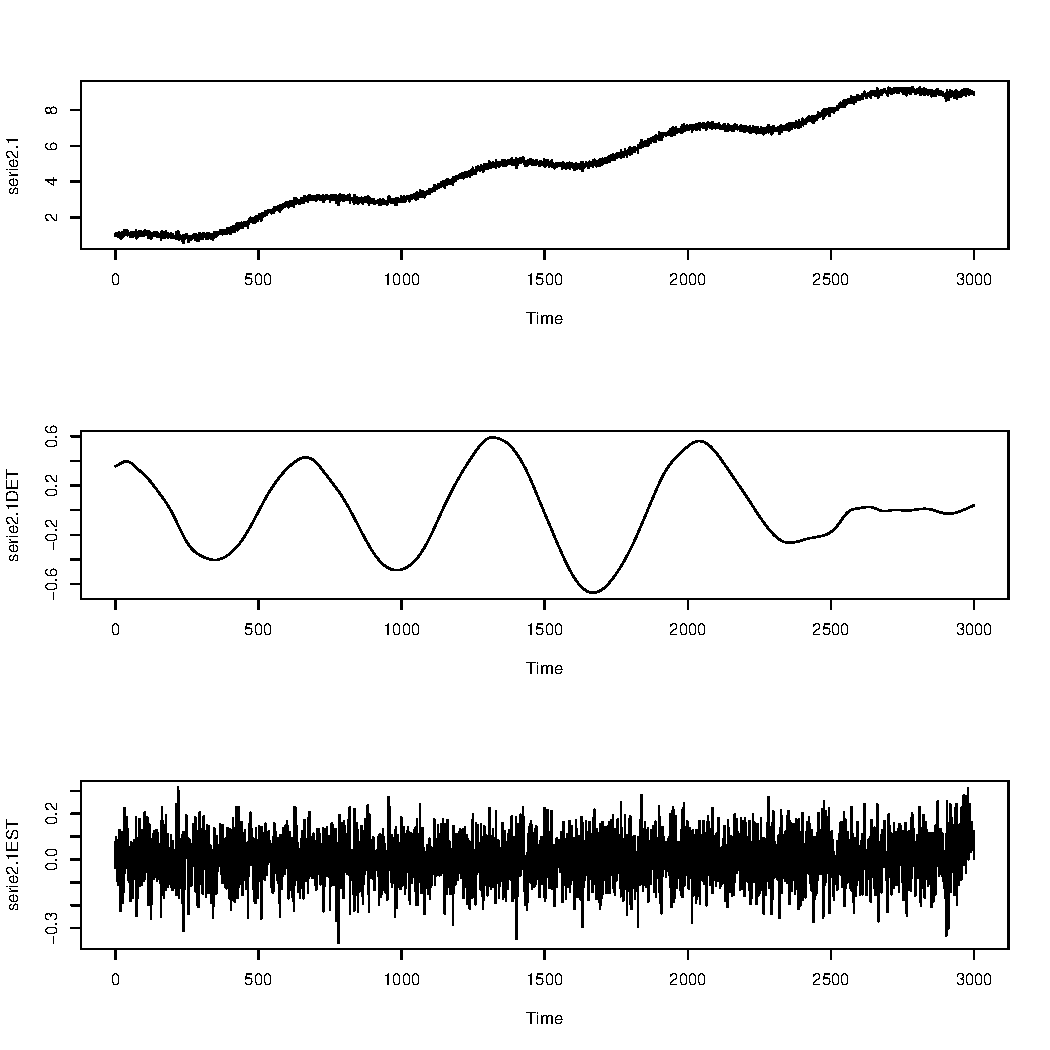
\includegraphics[scale=0.43]{serie2_1.pdf} \quad
  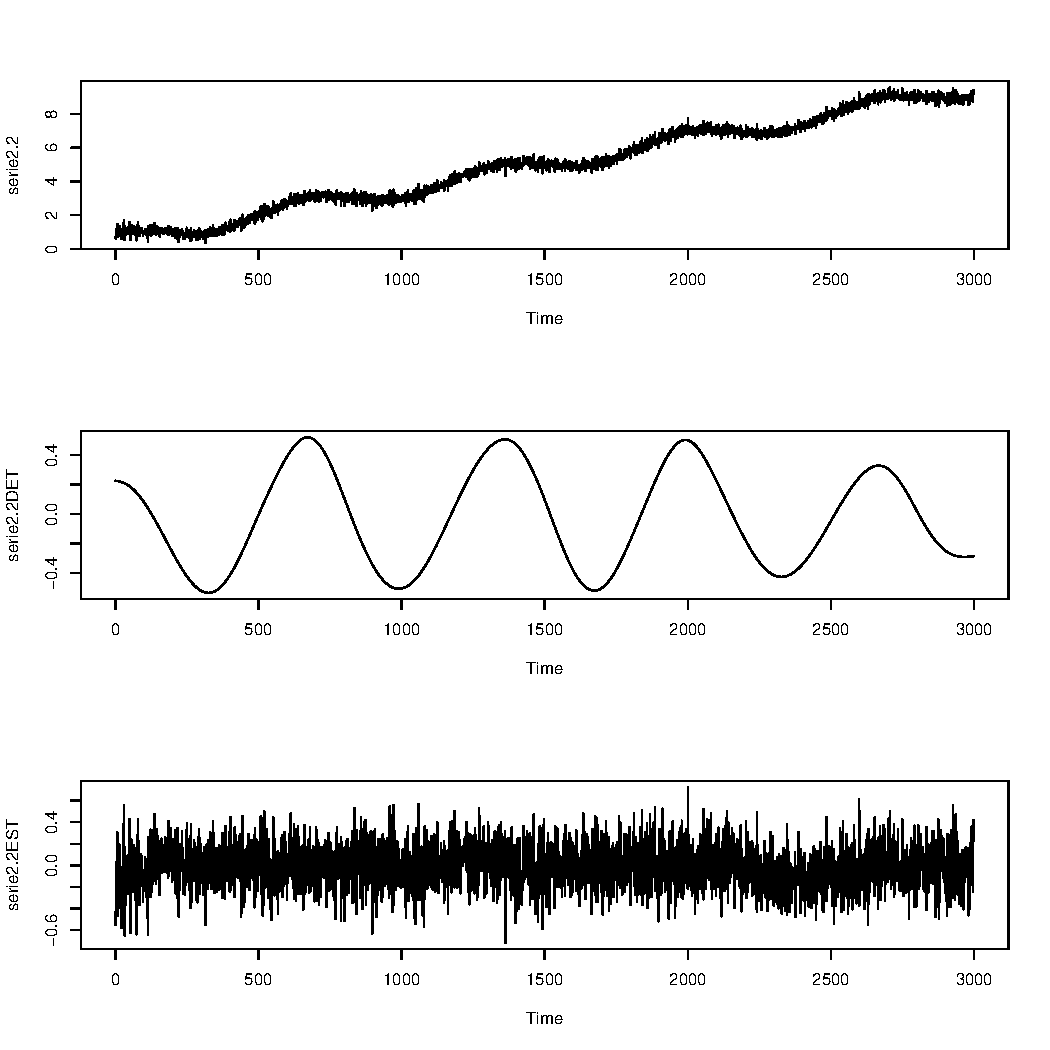
\includegraphics[scale=0.43]{serie2_2.pdf}
  \caption{Série 2.1 e Série 2.2}

\end{center}
\end{figure}

\graphicspath{{imagens/}}
\begin{figure}[H]
\begin{center}
  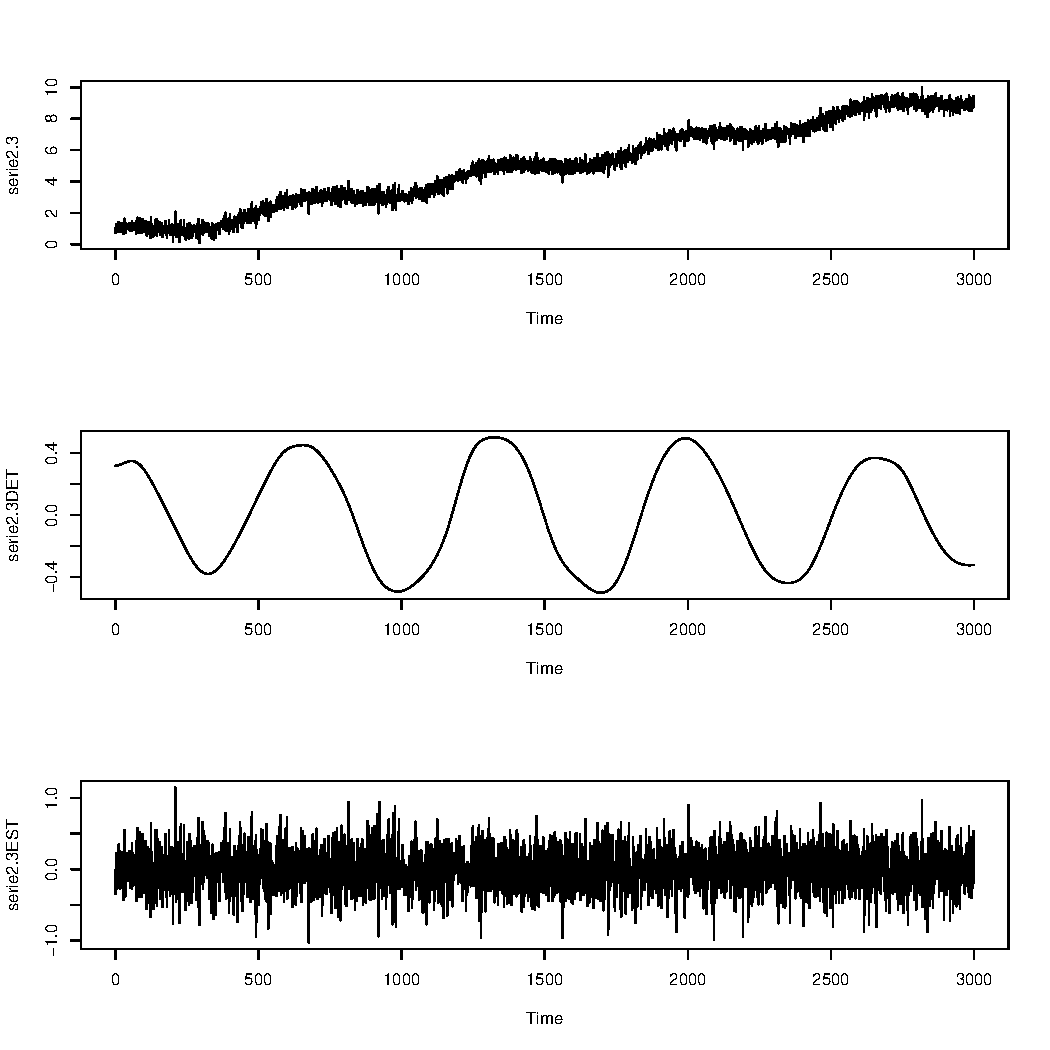
\includegraphics[scale=0.43]{serie2_3.pdf} \quad
  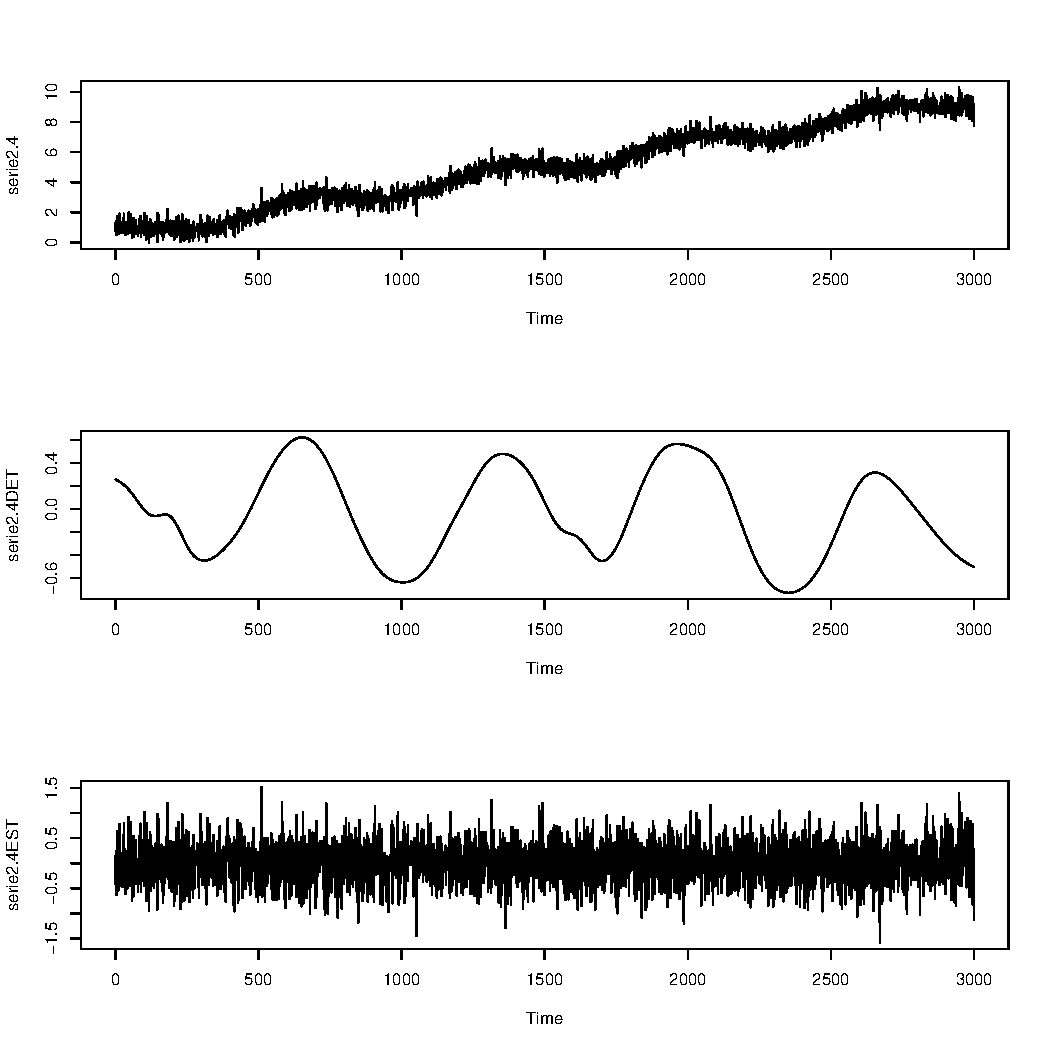
\includegraphics[scale=0.43]{serie2_4.pdf}
  \caption{Série 2.3 e Série 2.4}

\end{center}
\end{figure}

\graphicspath{{imagens/}}
\begin{figure}[H]
\begin{center}
  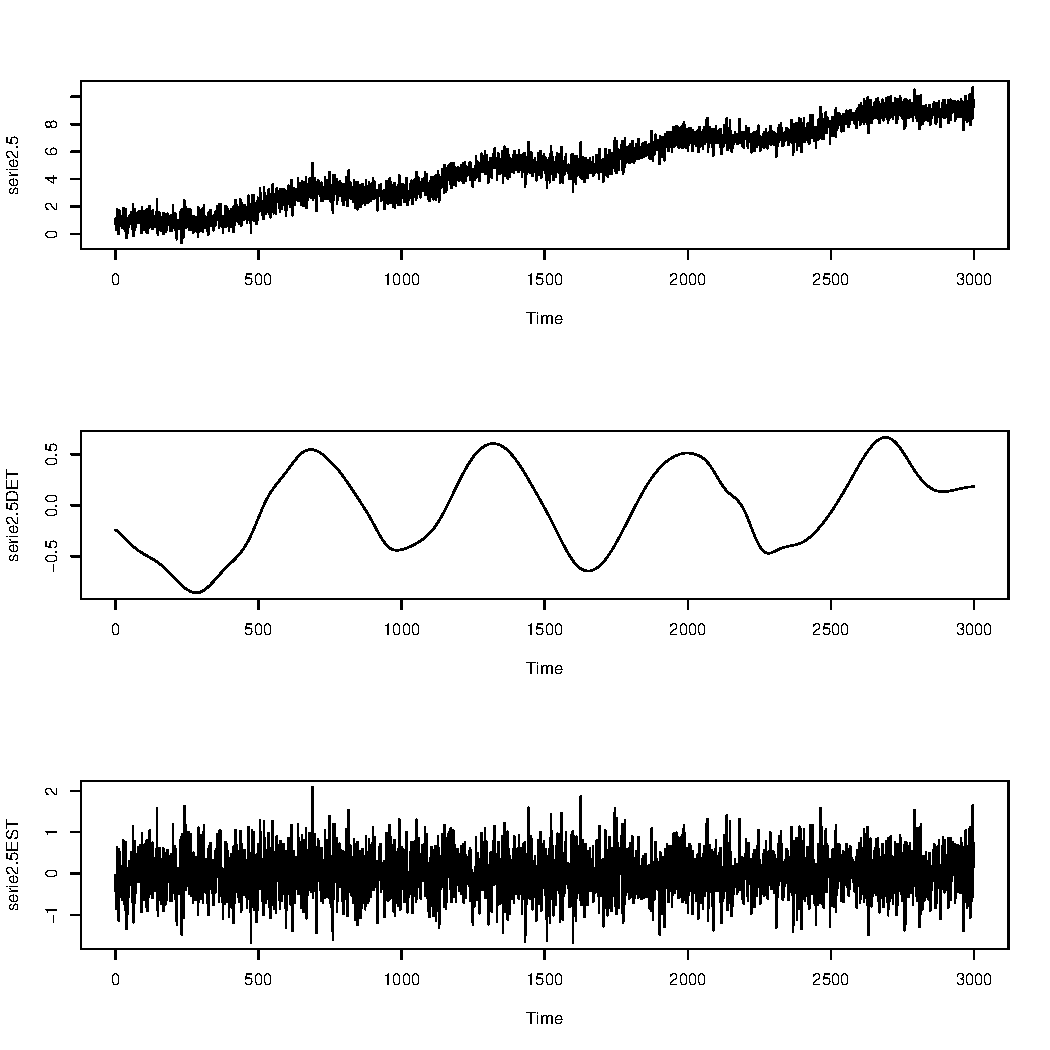
\includegraphics[scale=0.43]{serie2_5.pdf} \quad
  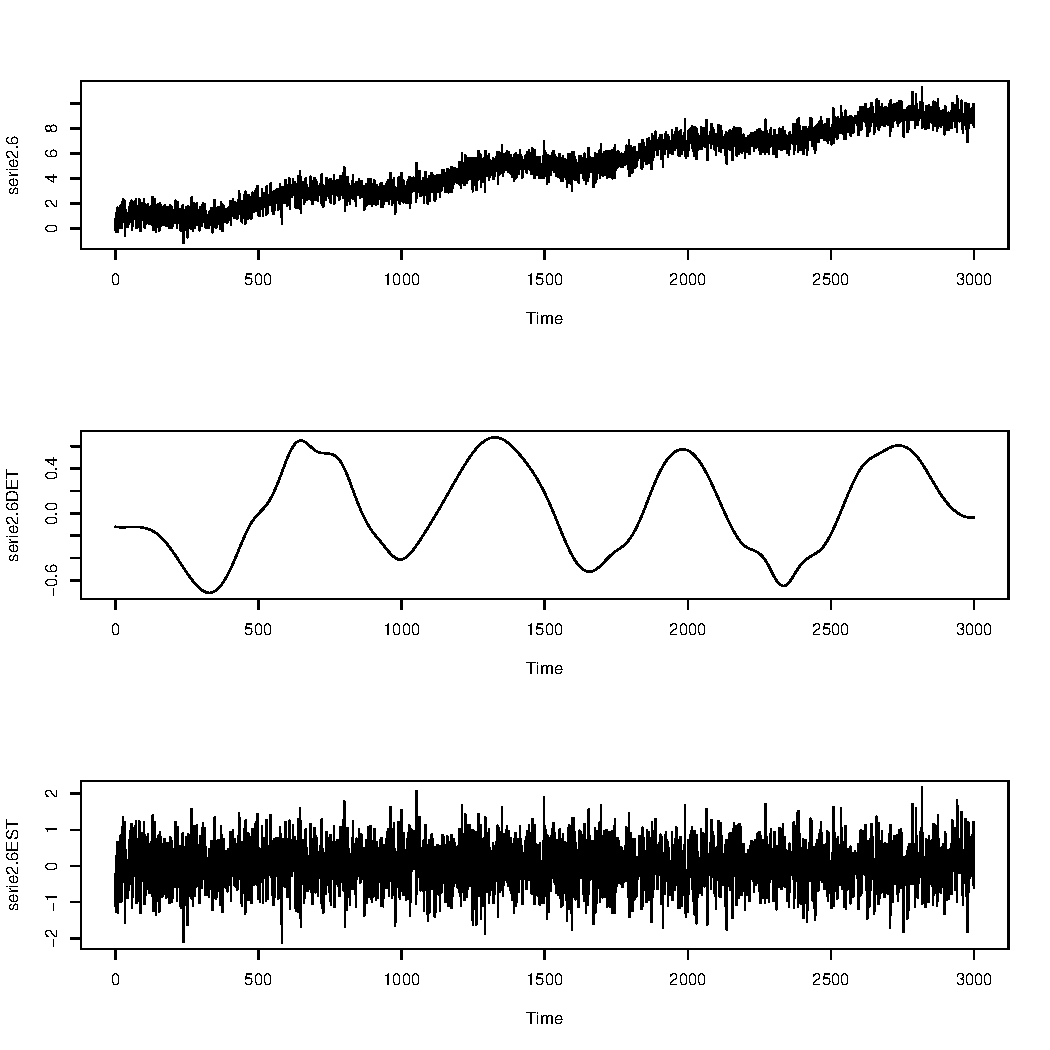
\includegraphics[scale=0.43]{serie2_6.pdf}
  \caption{Série 2.5 e Série 2.6}

\end{center}
\end{figure}

\graphicspath{{imagens/}}
\begin{figure}[H]
\begin{center}
  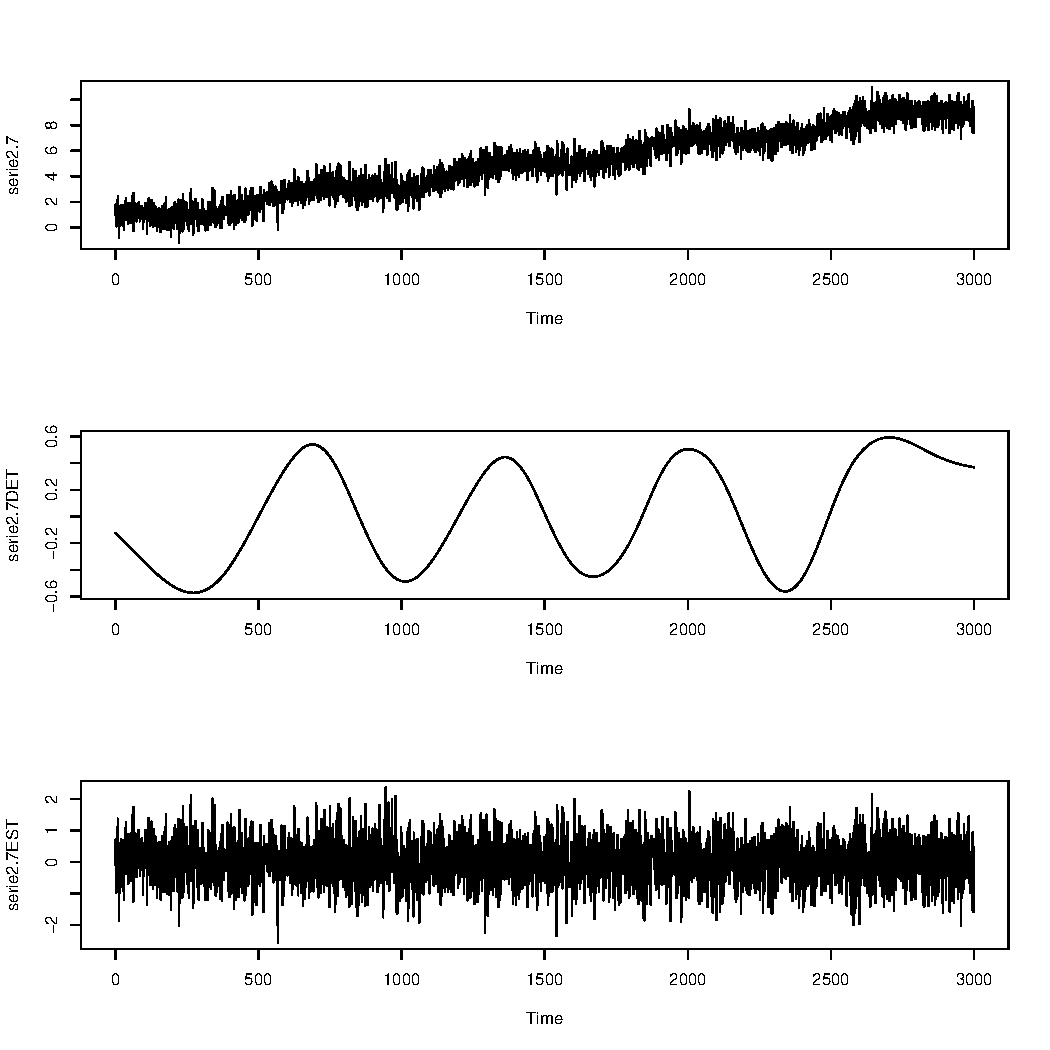
\includegraphics[scale=0.43]{serie2_7.pdf} \quad
  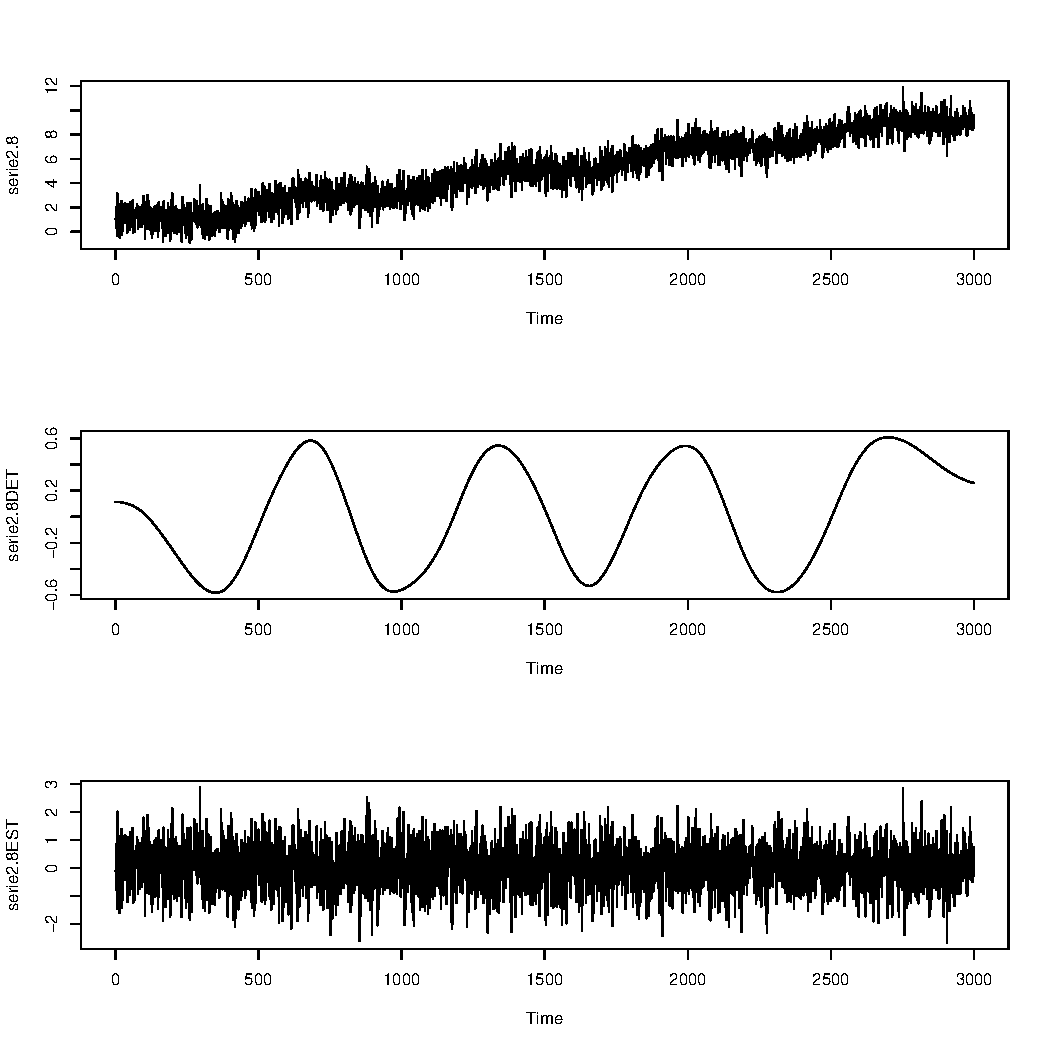
\includegraphics[scale=0.43]{serie2_8.pdf}
  \caption{Série 2.7 e Série 2.8}

\end{center}
\end{figure}

\graphicspath{{imagens/}}
\begin{figure}[H]
\begin{center}
  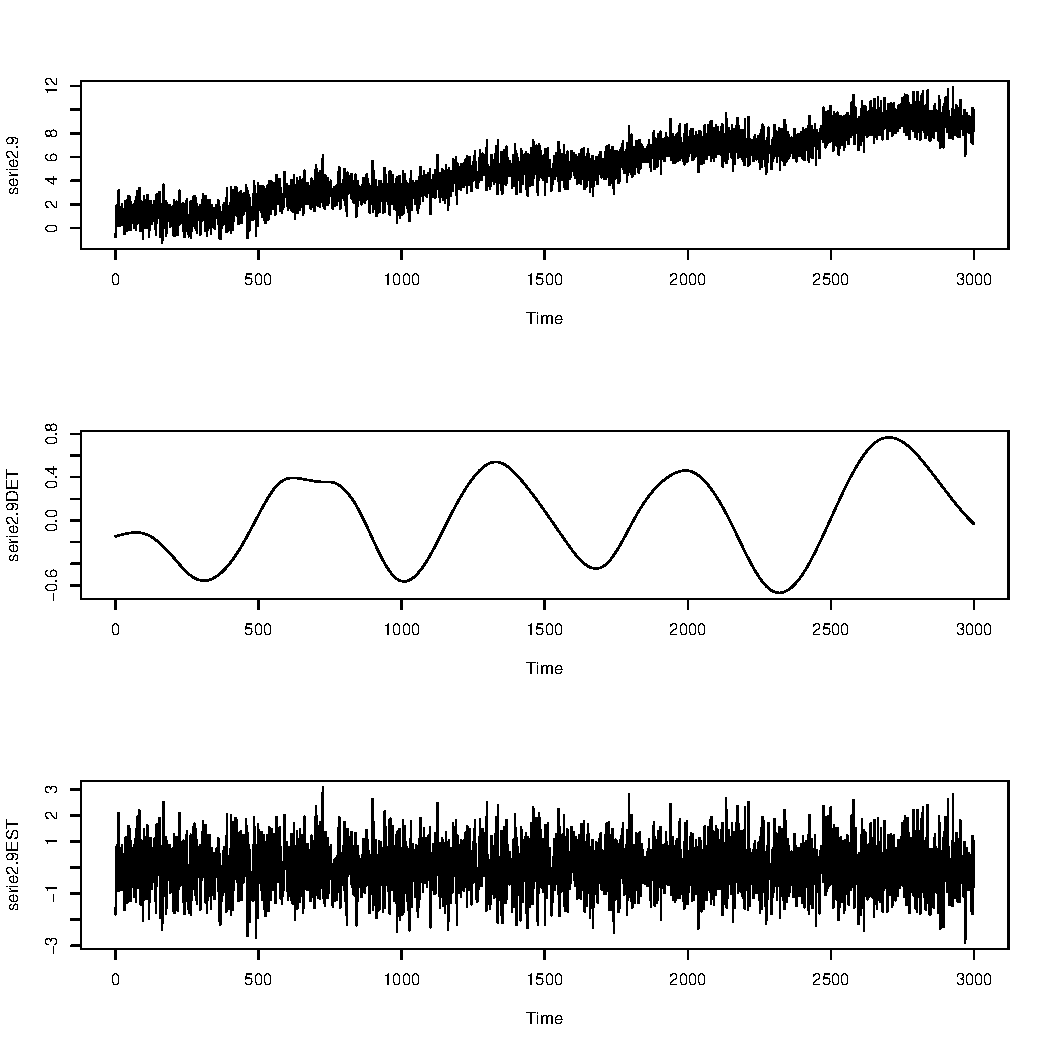
\includegraphics[scale=0.43]{serie2_9.pdf} \quad
  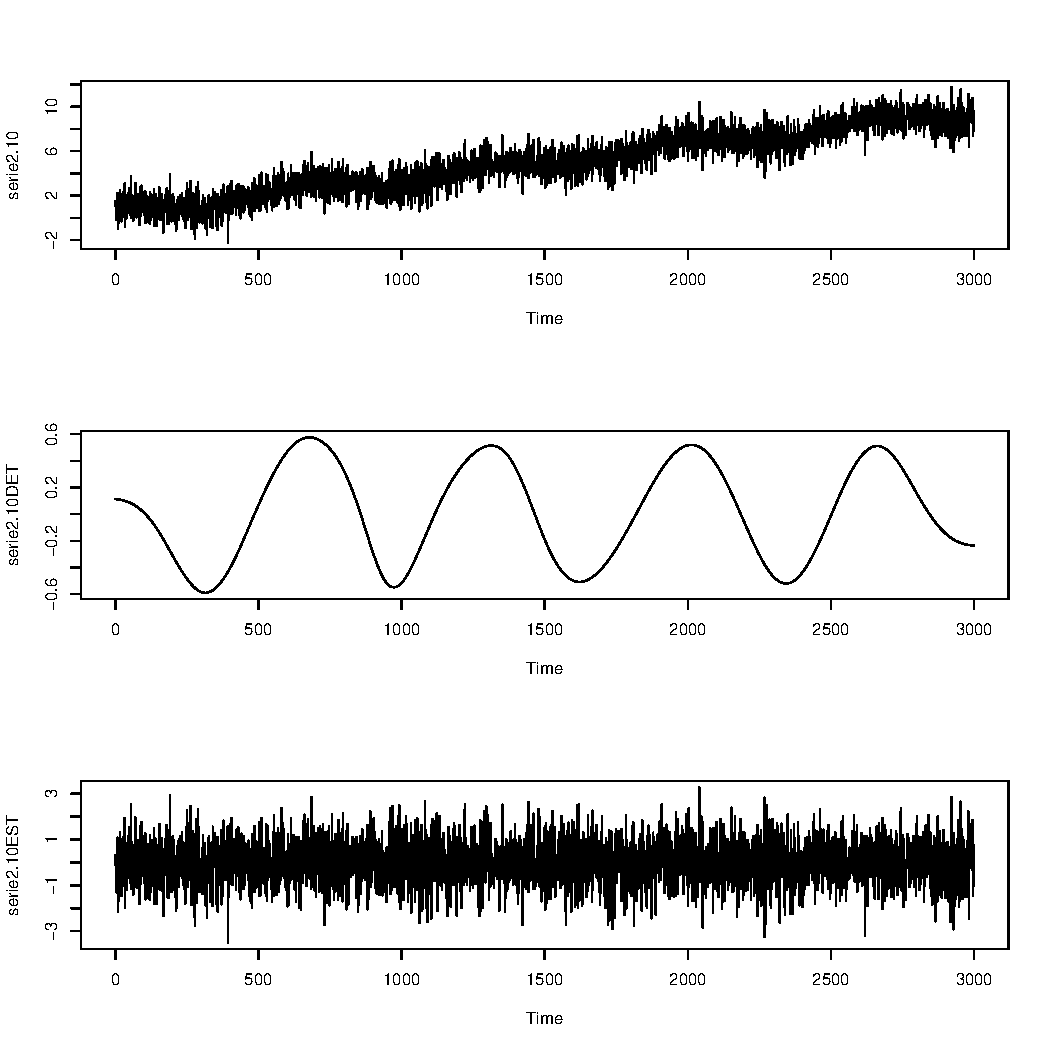
\includegraphics[scale=0.43]{serie2_10.pdf}
  \caption{Série 2.9 e Série 2.10}

\end{center}
\end{figure}

\section{Séries TIPO 3}
10 séries senoide com ruído ao longo da série.
\graphicspath{{imagens/}}
\begin{figure}[H]
\begin{center}
  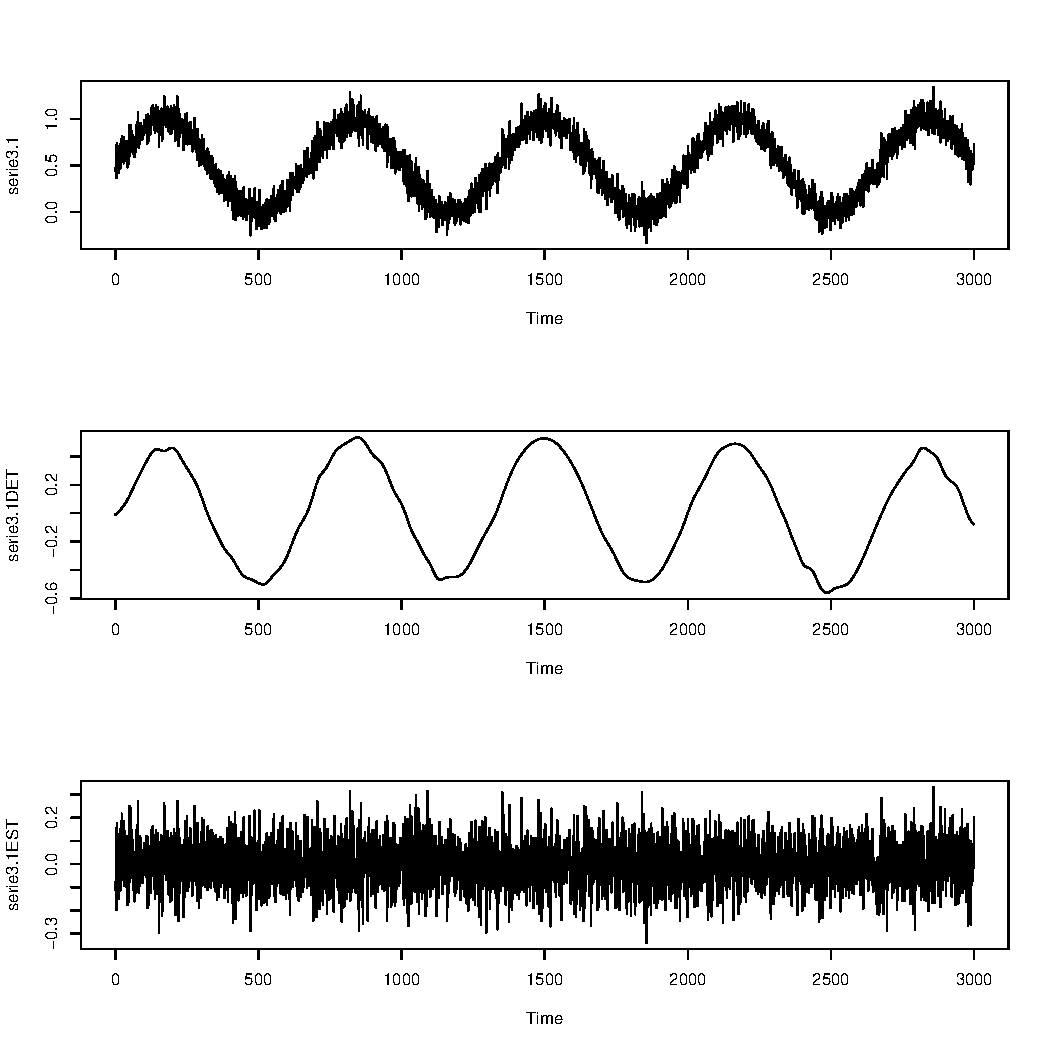
\includegraphics[scale=0.43]{serie3_1.pdf} \quad
  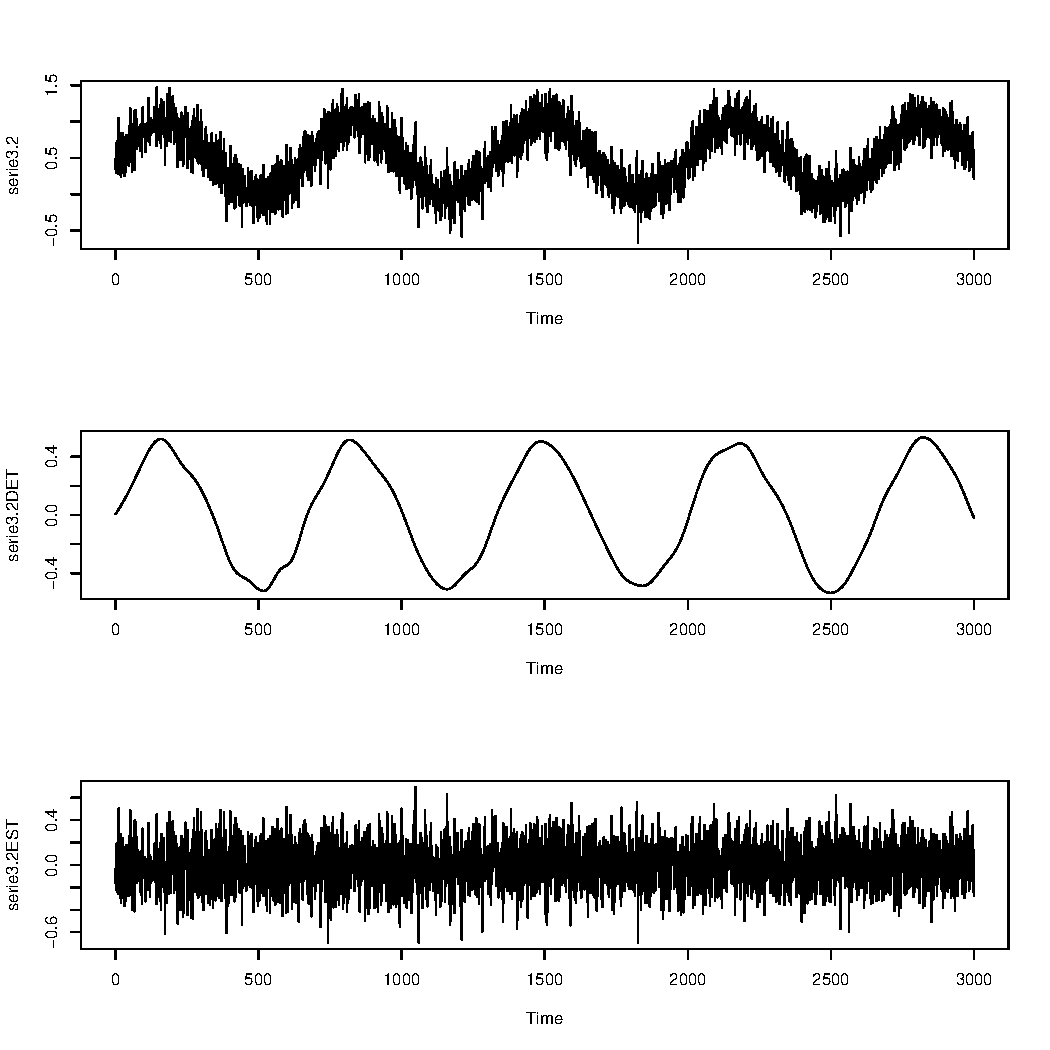
\includegraphics[scale=0.43]{serie3_2.pdf}
  \caption{Série 3.1 e Série 3.2}

\end{center}
\end{figure}

\graphicspath{{imagens/}}
\begin{figure}[H]
\begin{center}
  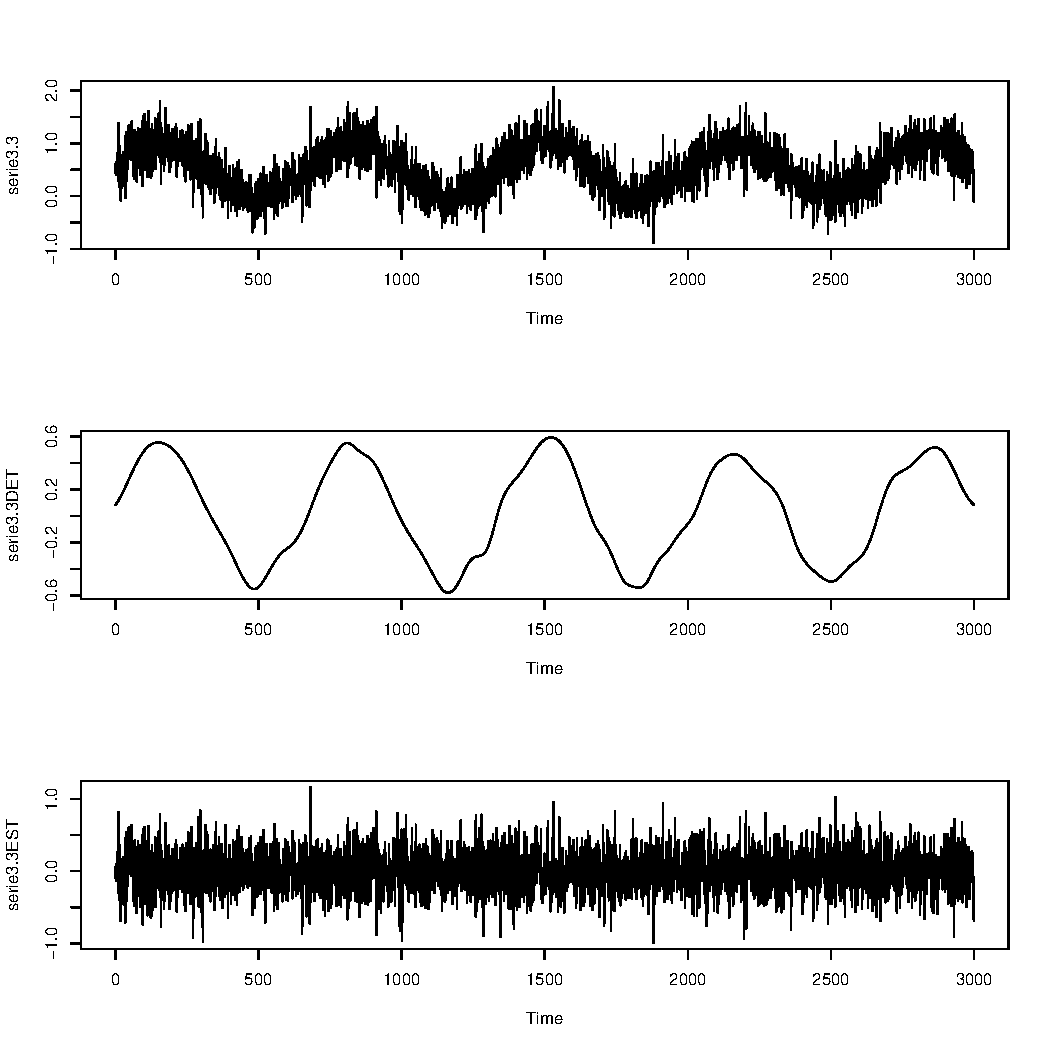
\includegraphics[scale=0.43]{serie3_3.pdf} \quad
  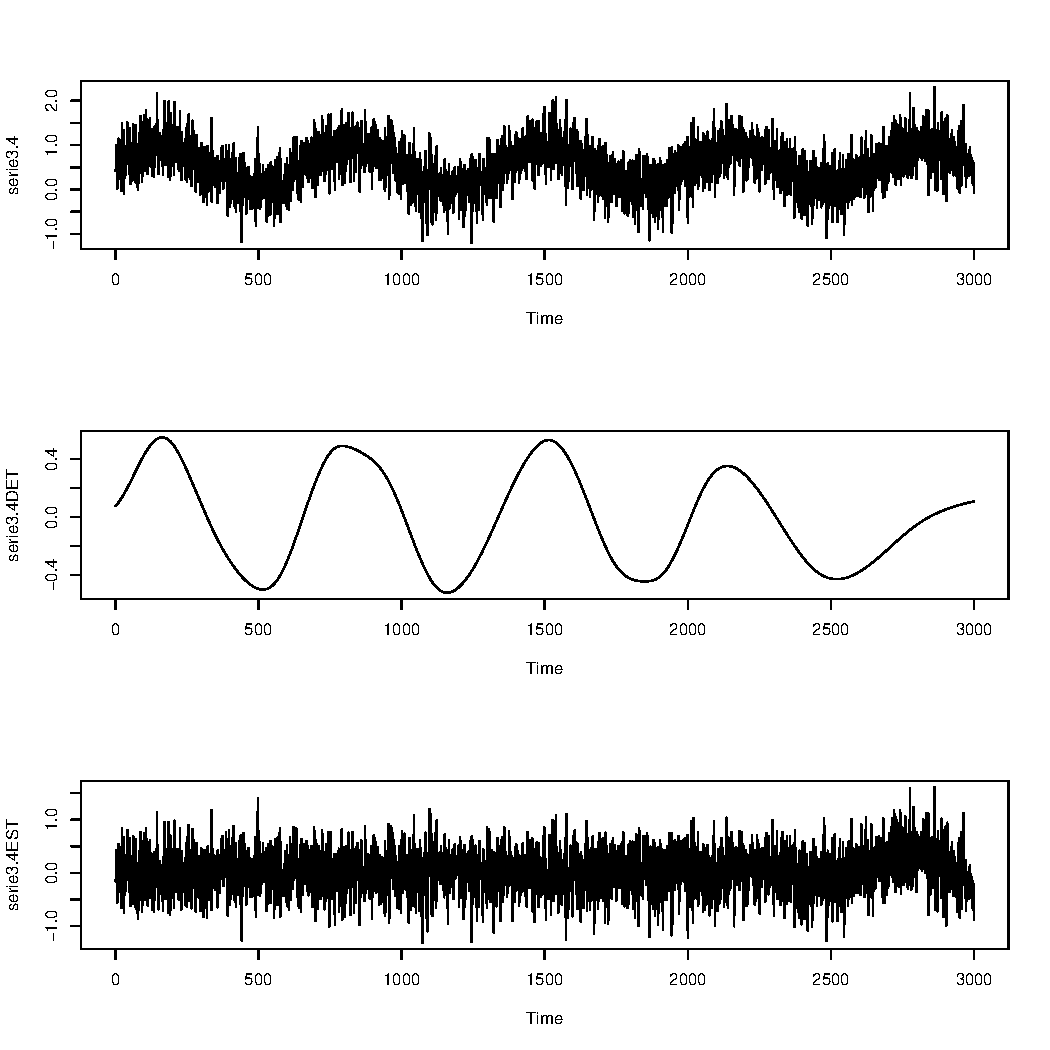
\includegraphics[scale=0.43]{serie3_4.pdf}
  \caption{Série 3.3 e Série 3.4}

\end{center}
\end{figure}

\graphicspath{{imagens/}}
\begin{figure}[H]
\begin{center}
  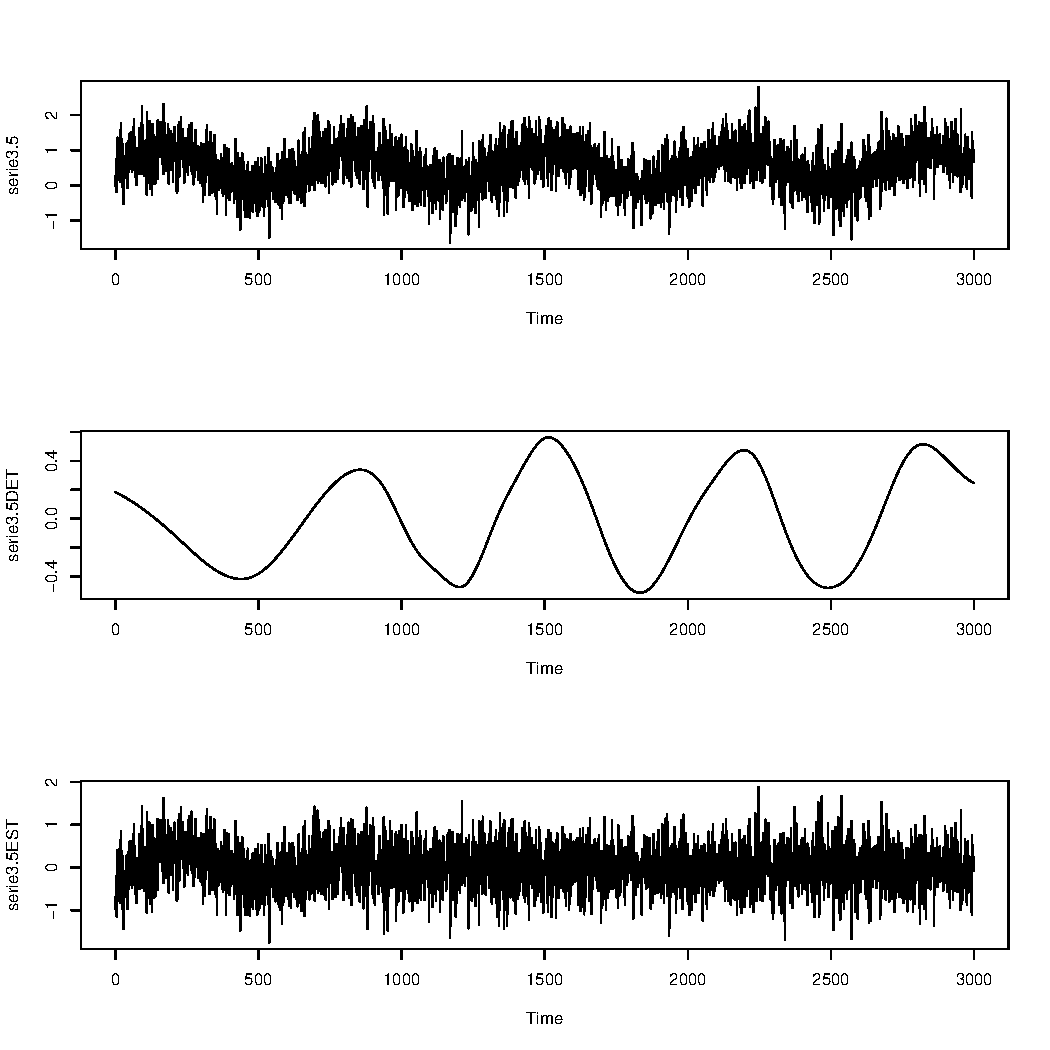
\includegraphics[scale=0.43]{serie3_5.pdf} \quad
  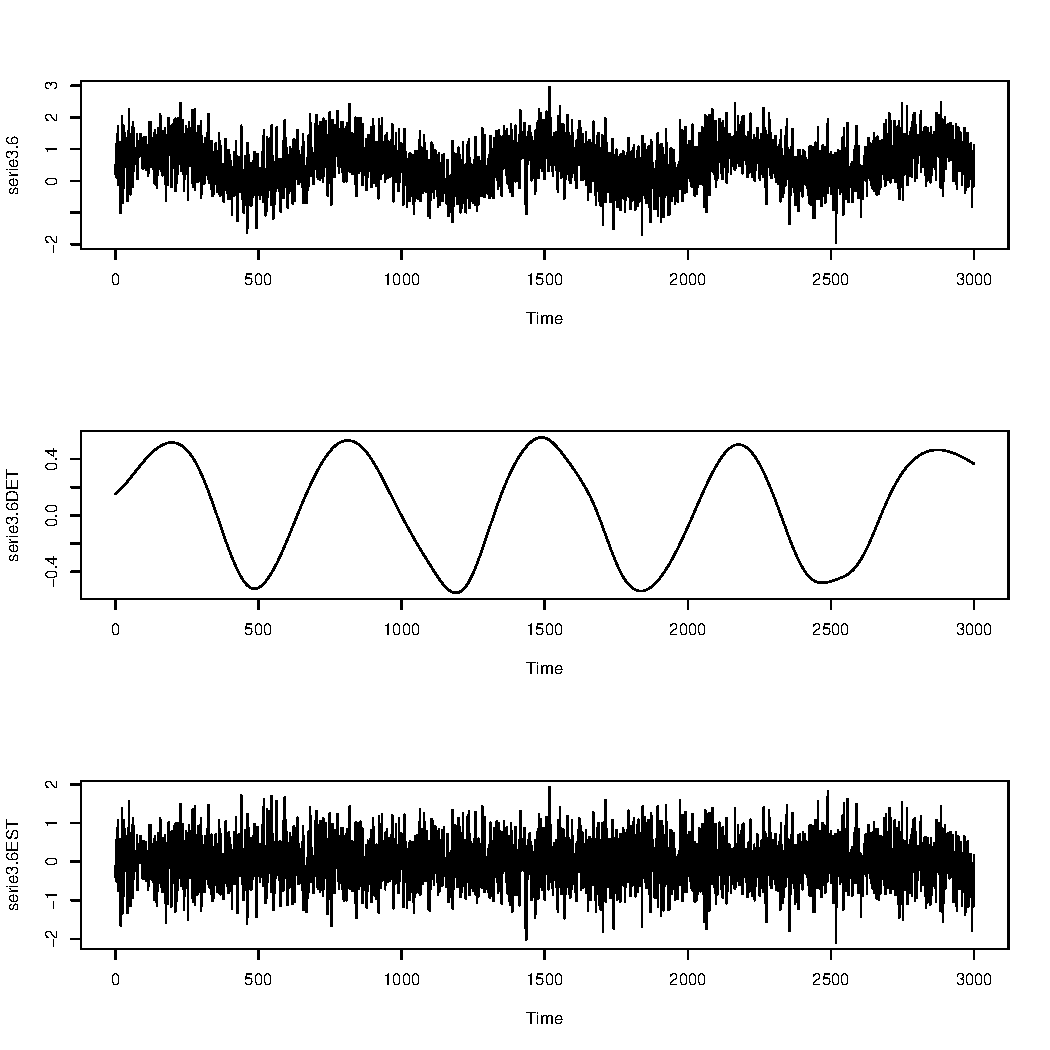
\includegraphics[scale=0.43]{serie3_6.pdf}
  \caption{Série 3.5 e Série 3.6}

\end{center}
\end{figure}

\graphicspath{{imagens/}}
\begin{figure}[H]
\begin{center}
  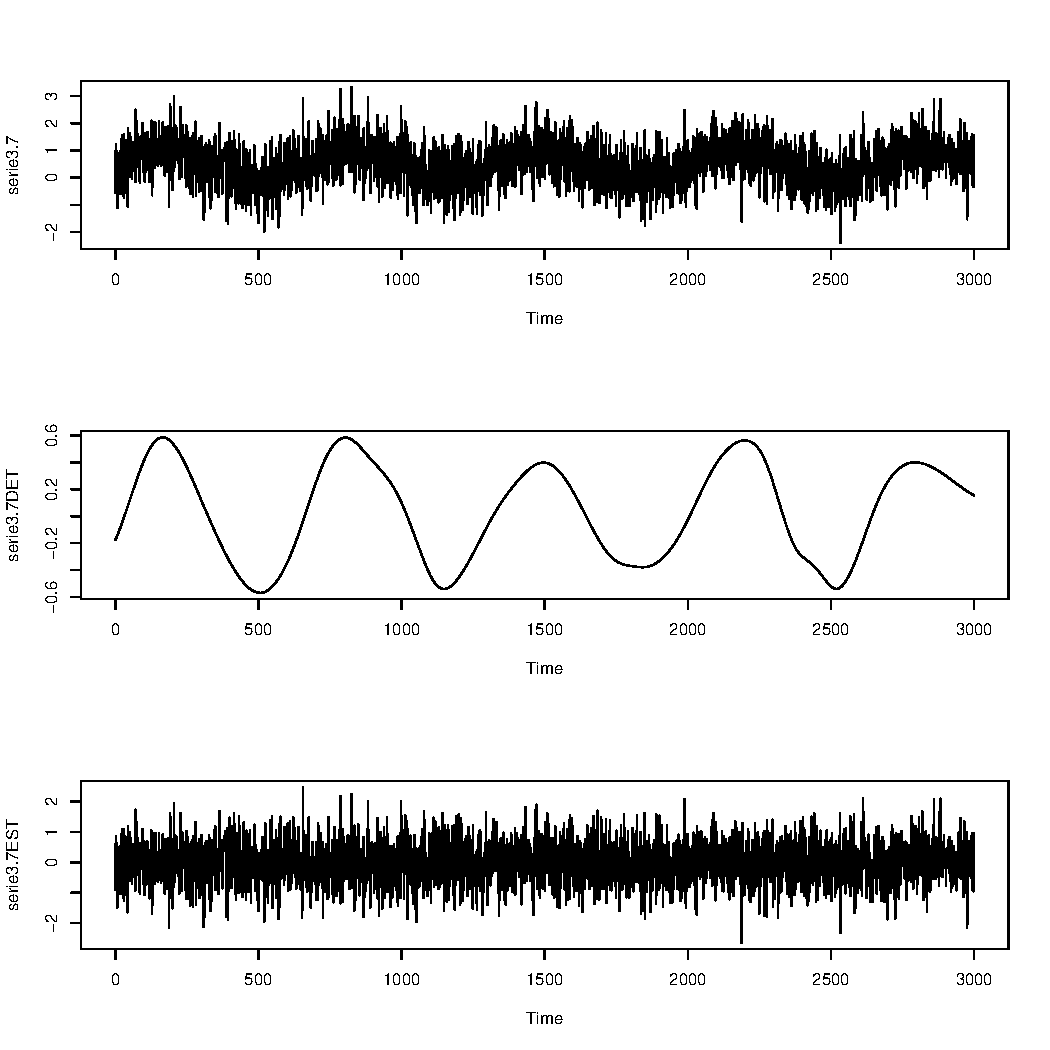
\includegraphics[scale=0.43]{serie3_7.pdf} \quad
  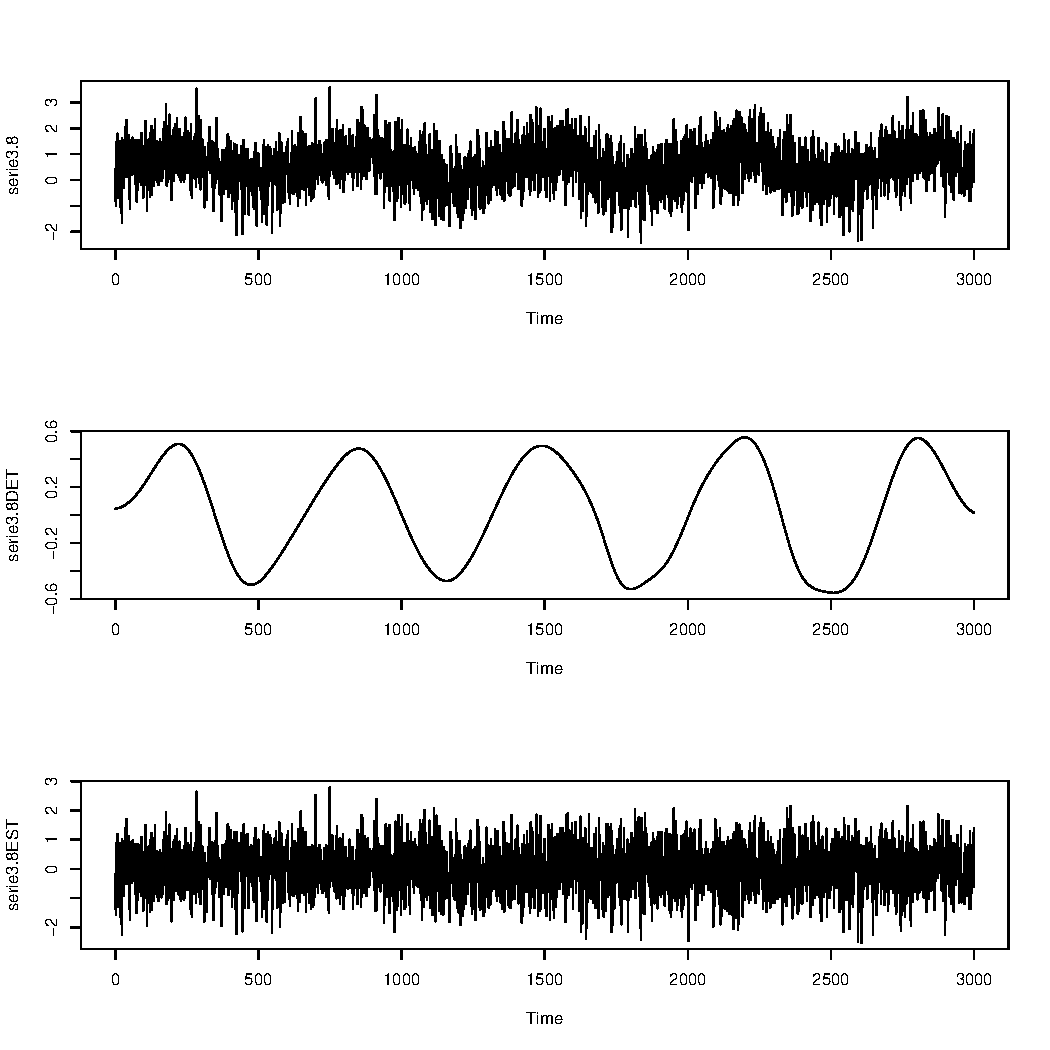
\includegraphics[scale=0.43]{serie3_8.pdf}
  \caption{Série 3.7 e Série 3.8}

\end{center}
\end{figure}

\graphicspath{{imagens/}}
\begin{figure}[H]
\begin{center}
  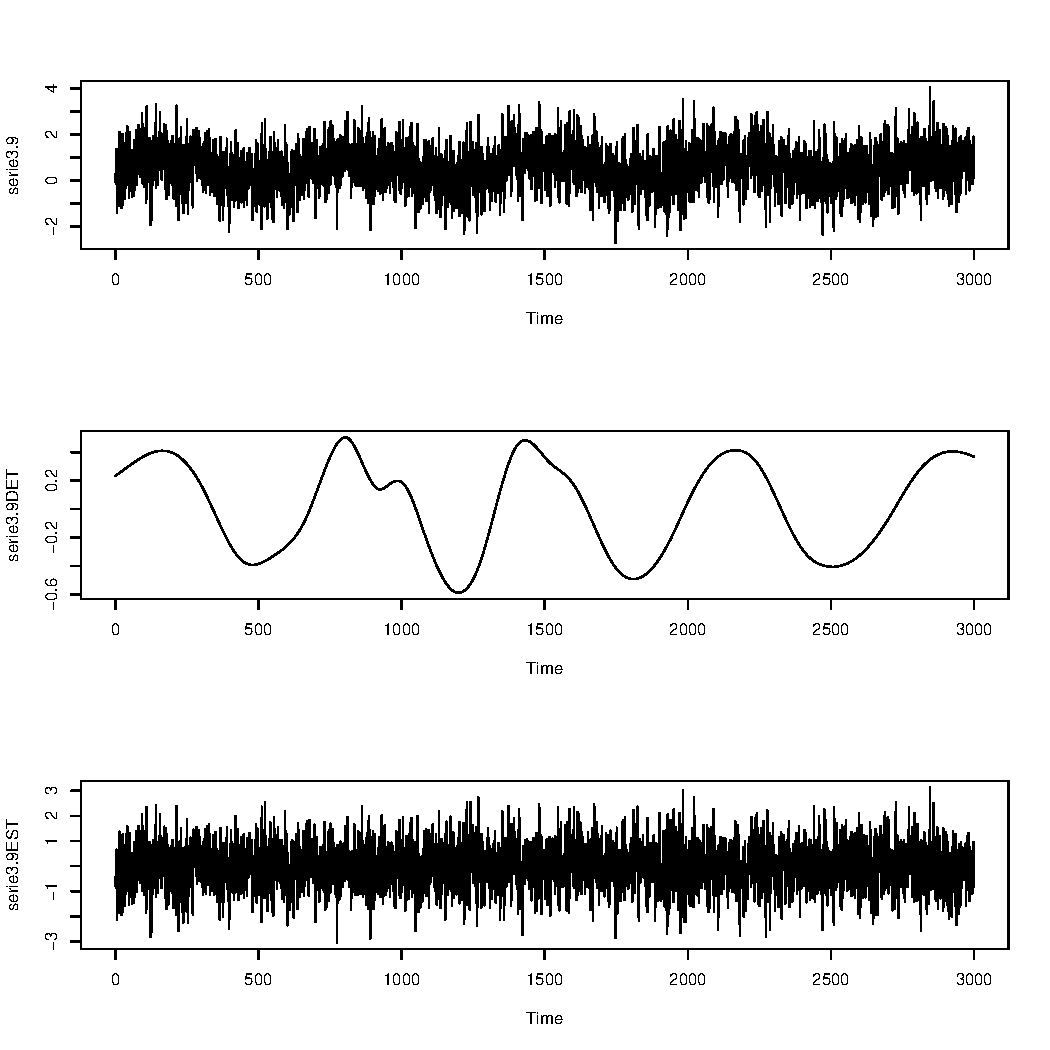
\includegraphics[scale=0.43]{serie3_9.pdf} \quad
  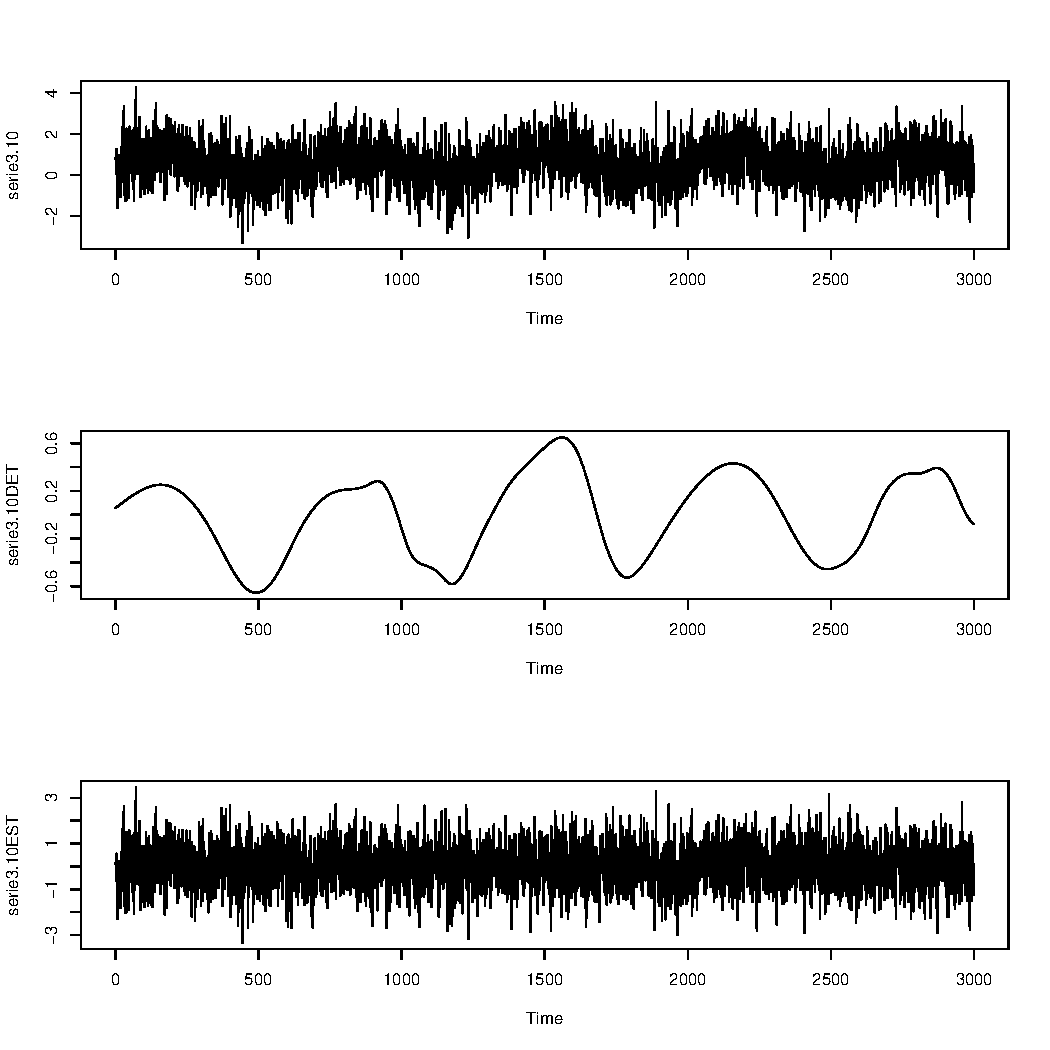
\includegraphics[scale=0.43]{serie3_10.pdf}
  \caption{Série 3.9 e Série 3.10}

\end{center}
\end{figure}

\section{Séries TIPO 4}
10 séries senoide com ruído ao longo da série e tendência.
\graphicspath{{imagens/}}
\begin{figure}[H]
\begin{center}
  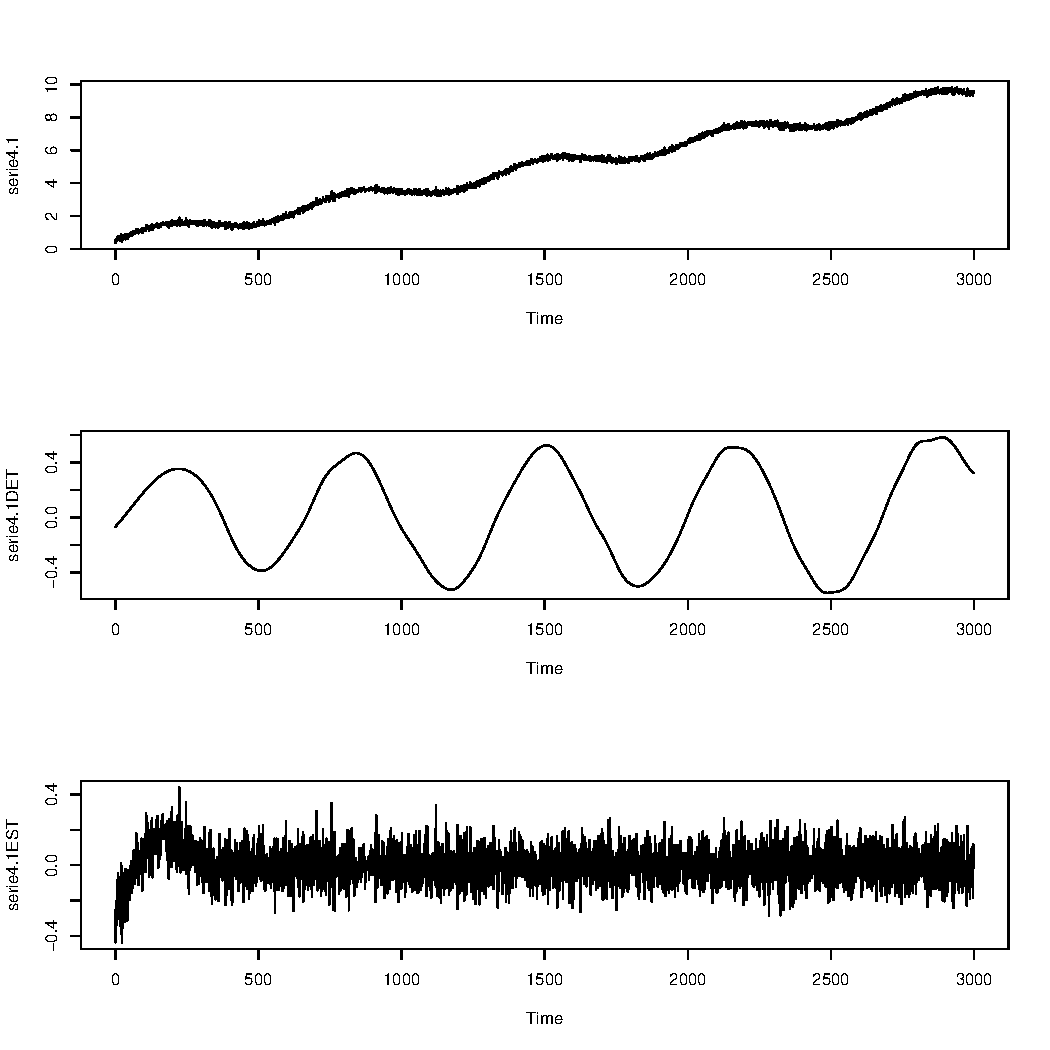
\includegraphics[scale=0.43]{serie4_1.pdf} \quad
  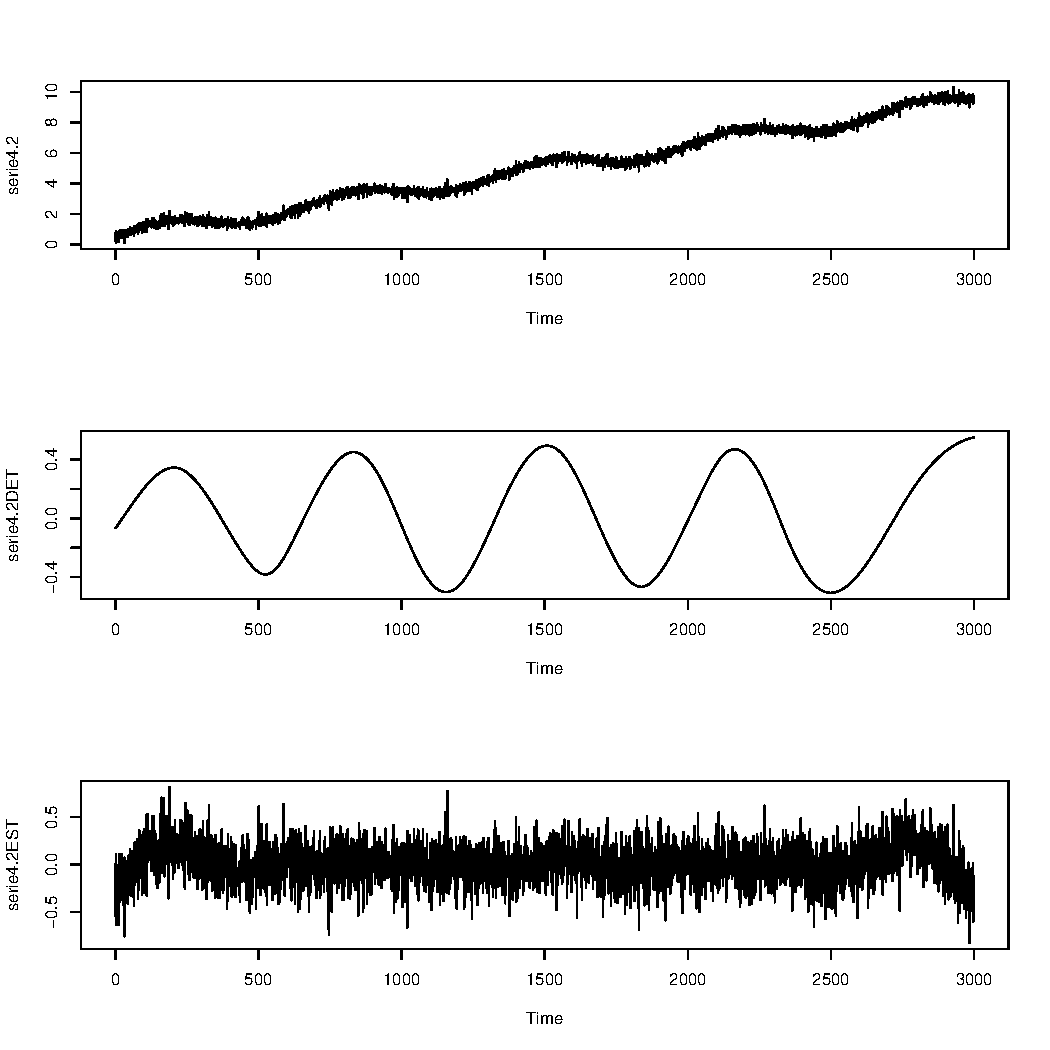
\includegraphics[scale=0.43]{serie4_2.pdf}
  \caption{Série 4.1 e Série 4.2}
\end{center}
\end{figure}

\graphicspath{{imagens/}}
\begin{figure}[H]
\begin{center}
  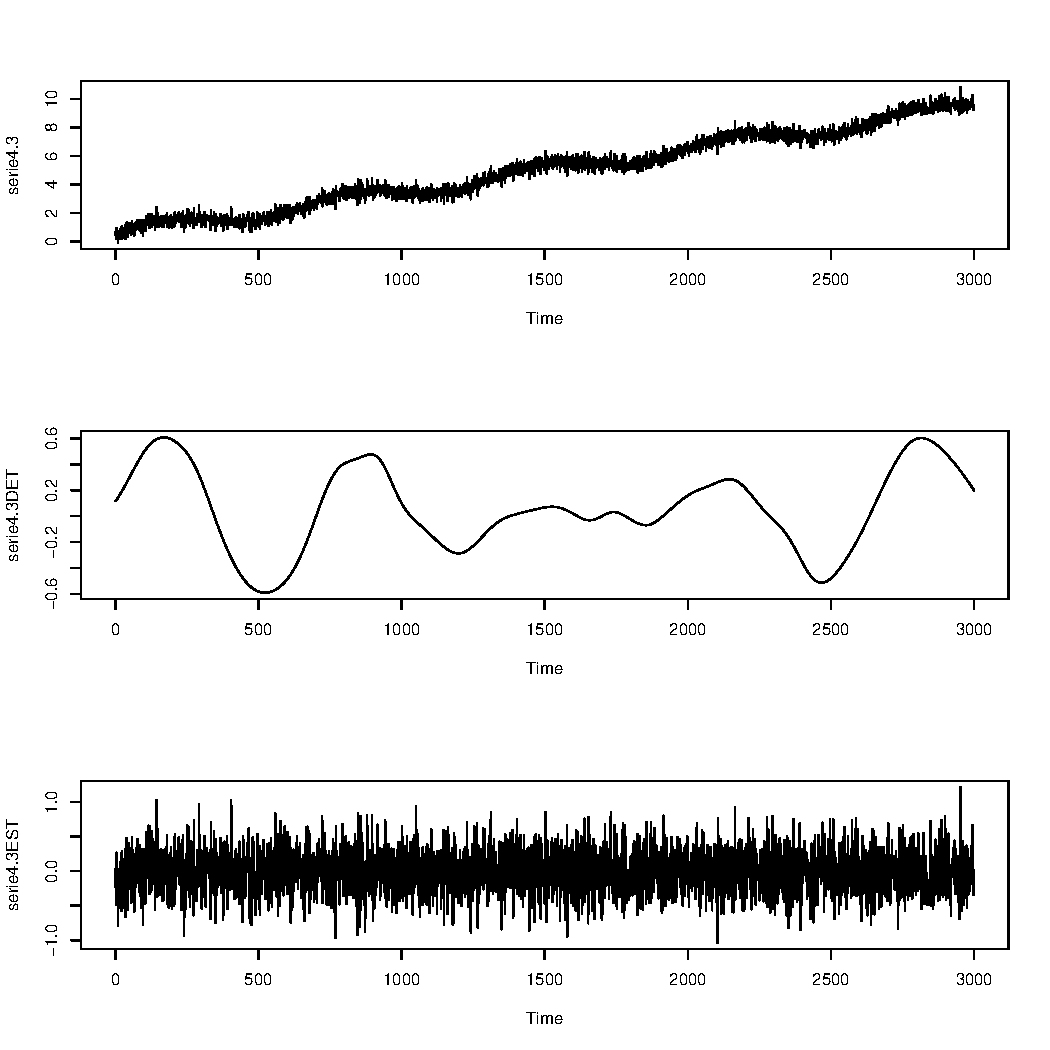
\includegraphics[scale=0.43]{serie4_3.pdf} \quad
 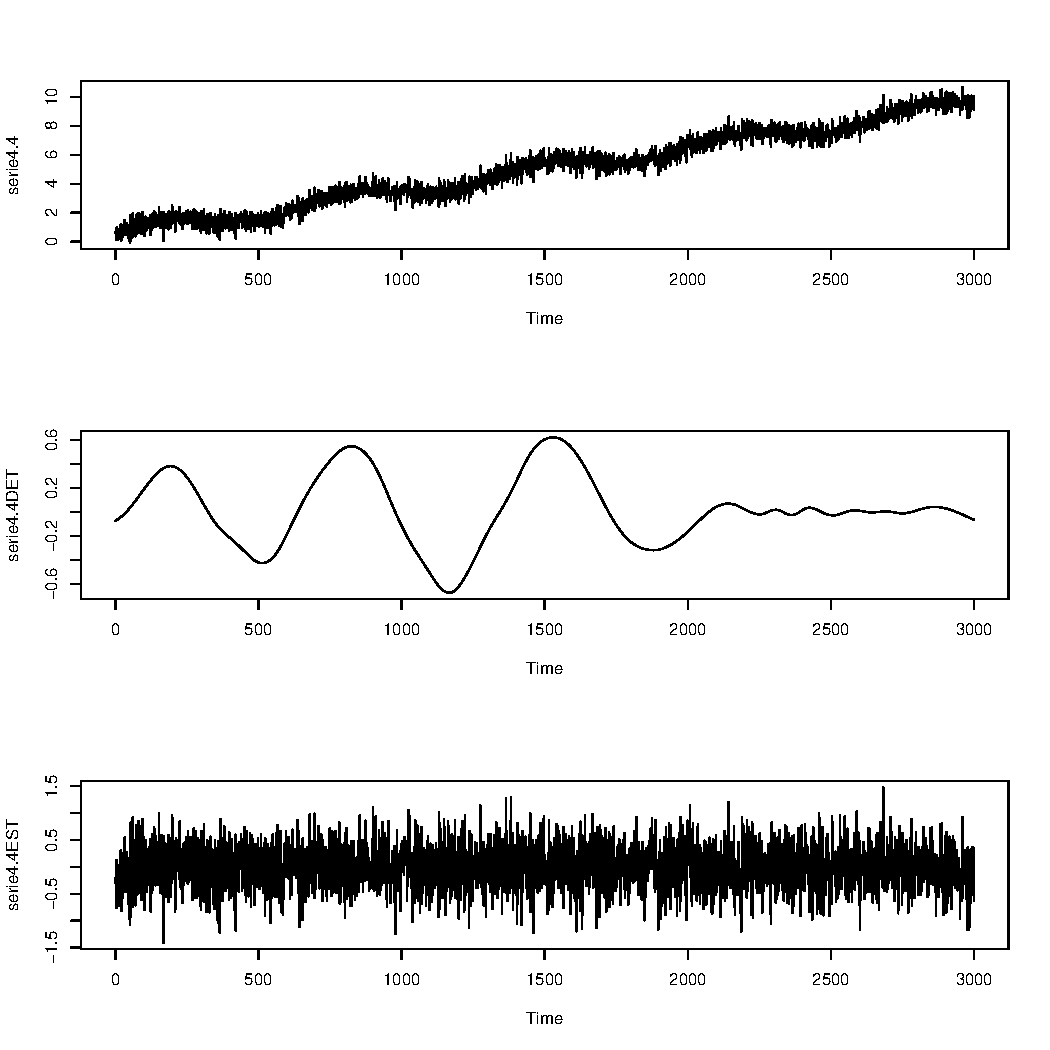
\includegraphics[scale=0.43]{serie4_4.pdf}
 \caption{Série 4.3 e Série 4.4}

\end{center}
\end{figure}

\graphicspath{{imagens/}}
\begin{figure}[H]
\begin{center}
  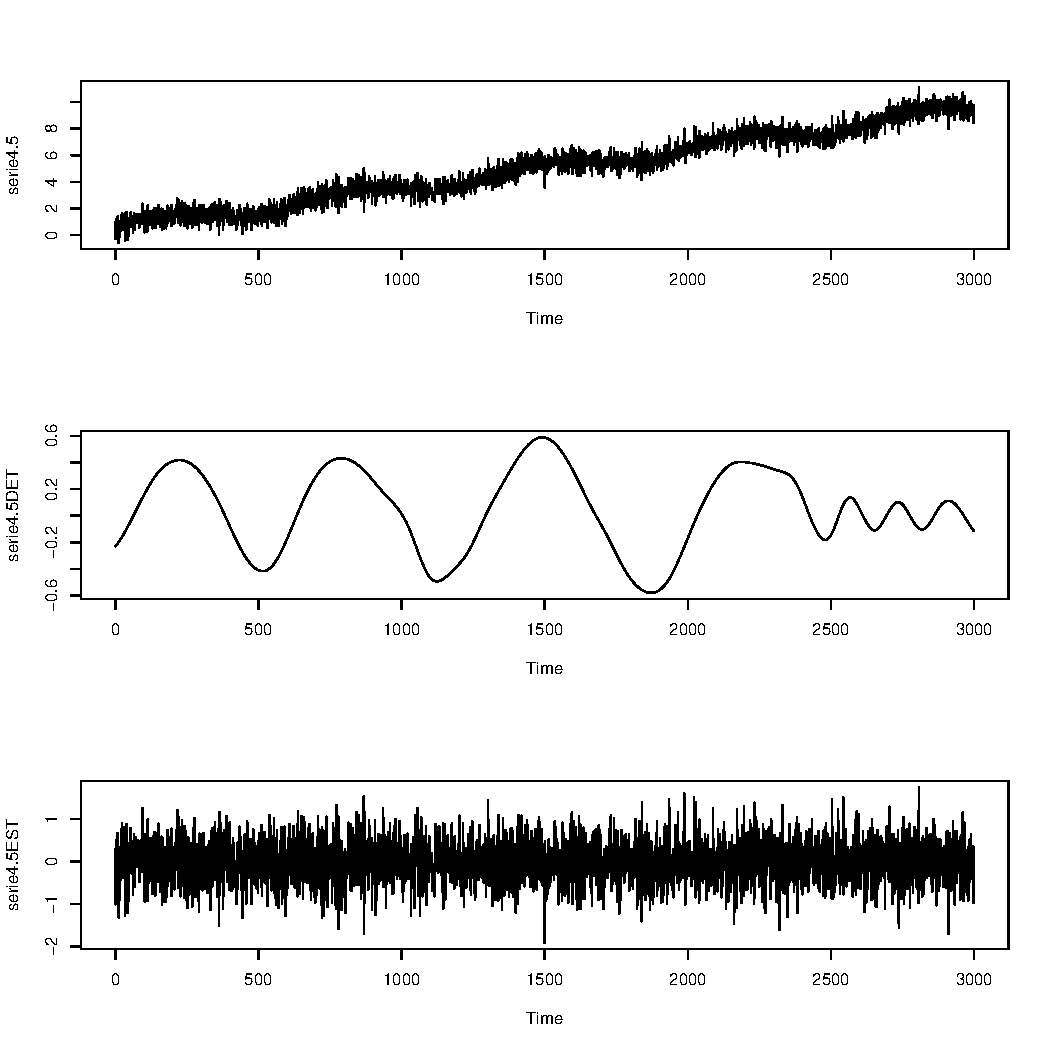
\includegraphics[scale=0.43]{serie4_5.pdf} \quad
  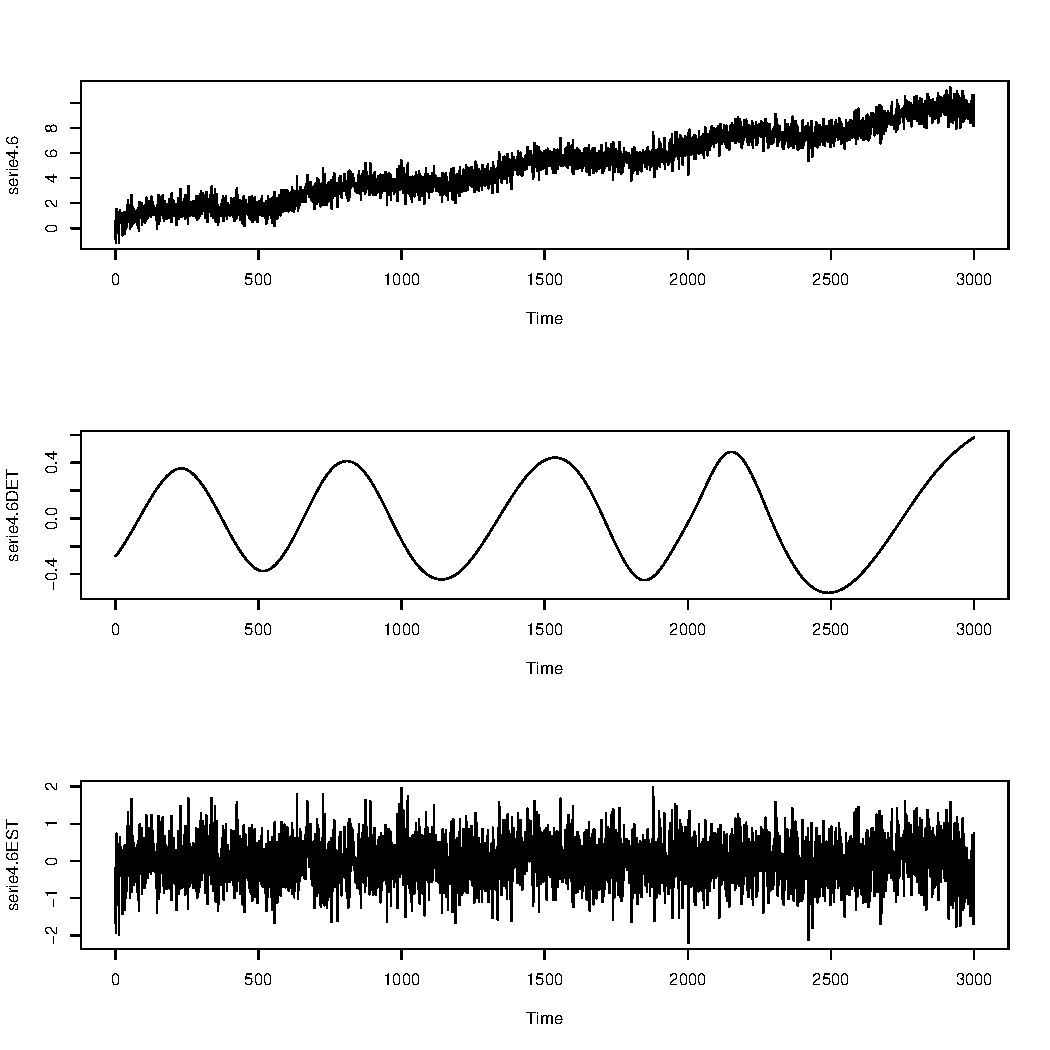
\includegraphics[scale=0.43]{serie4_6.pdf}
 \caption{Série 4.5 e Série 4.6}

\end{center}
\end{figure}

\graphicspath{{imagens/}}
\begin{figure}[H]
\begin{center}
  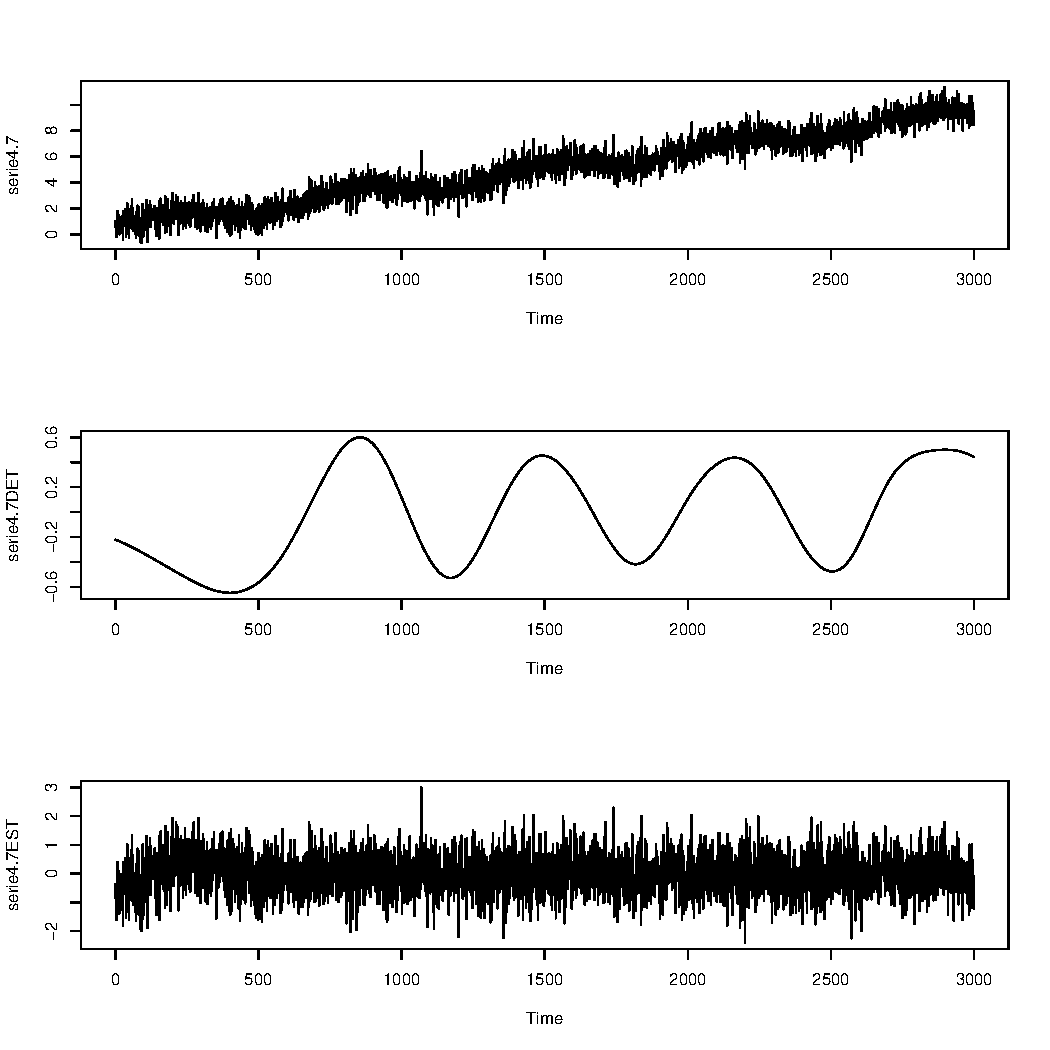
\includegraphics[scale=0.43]{serie4_7.pdf} \quad
  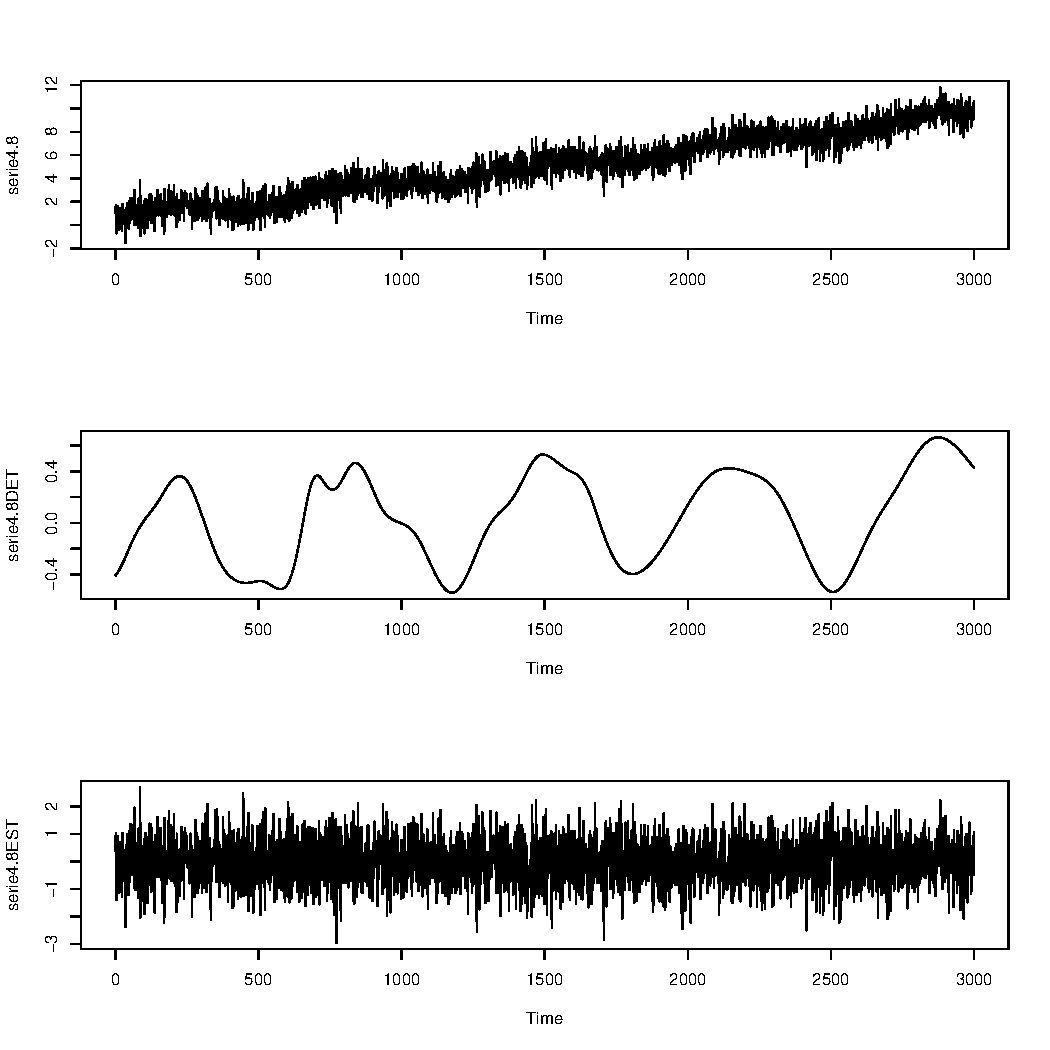
\includegraphics[scale=0.43]{serie4_8.pdf}
  \caption{Série 4.7 e Série 4.8}

\end{center}
\end{figure}

\graphicspath{{imagens/}}
\begin{figure}[H]
\begin{center}
  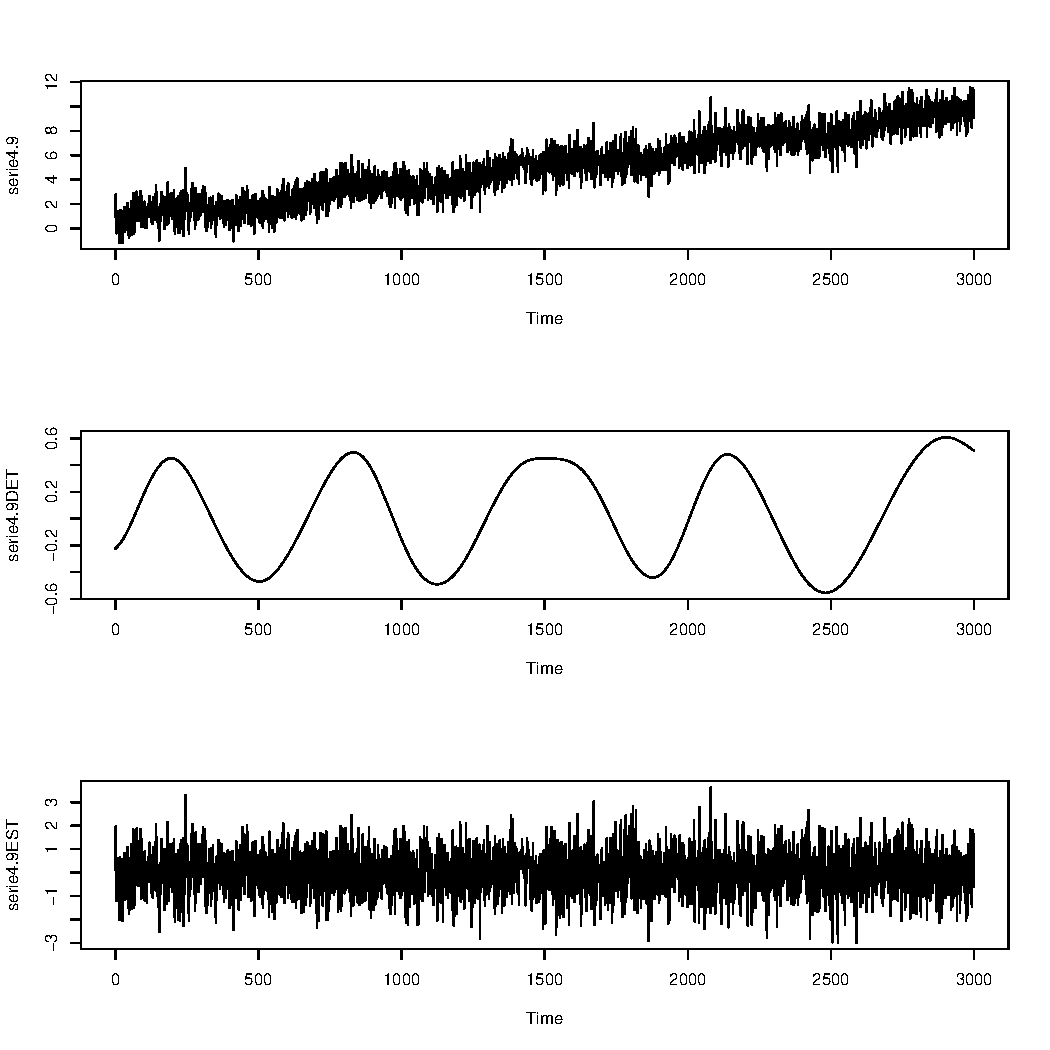
\includegraphics[scale=0.43]{serie4_9.pdf} \quad
  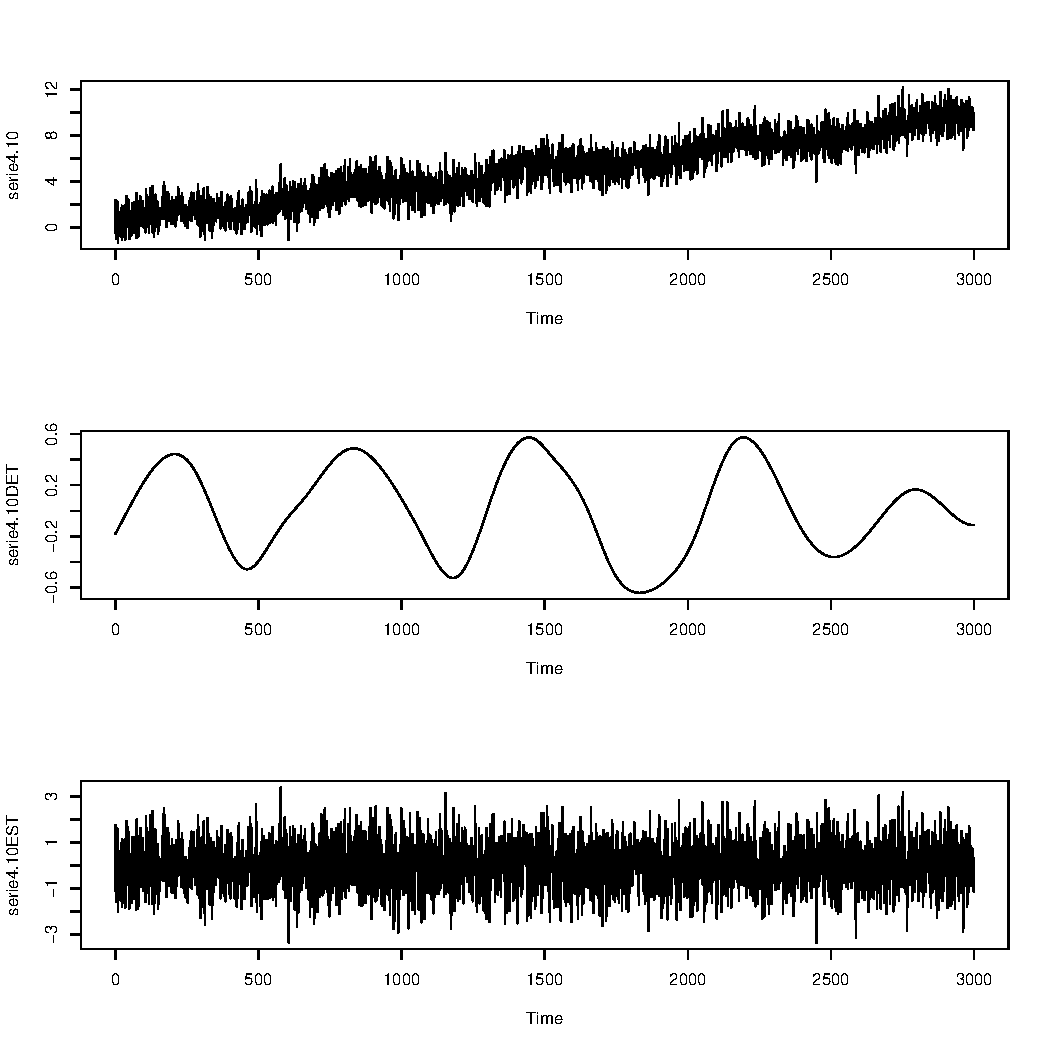
\includegraphics[scale=0.43]{serie4_10.pdf}
  \caption{Série 4.9 e Série 4.10}
\end{center}
\end{figure}
\section{Considerações Finais}
Foram apresentadas as séries temporais utilizadas neste trabalho experimental e suas respactivas decomposições.
% \include{apendice2}
% ...
% \include{apendiceM}

%% Fim do documento
\end{document}
%------------------------------------------------------------------------------------------%
